\section{Fundamentals of Particle Image Velocimetry}

Particle Image Velocimetry, or PIV, is a class of methods employed by 
experimental fluid mechanics to measure instantaneous vector velocity fields by 
measuring the displacements of small visible particles which follow the motion 
of the fluid. Figure \ref{fig:quiver_example} shows a typical 
resulting vector field from measurements of a vortical flow. Each of these 
two-dimensional vectors was measured simultaneously in a thin sheet of fluid. 
The velocity of the fluid is sensed by acquiring images of well entrained 
particles at precise times and measuring the displacement of those particles. 
This is accomplished with the use of cameras for acquiring images and an 
intense laser to illuminate particles within the desired plane. 
This technique can be used to study flows in gases and liquids, and is derived 
from techniques originally developed to measure deformations on the surface of 
solid material \cite{arroyo1991,adrian1991}.

\begin{figure}[H]
	\centering
	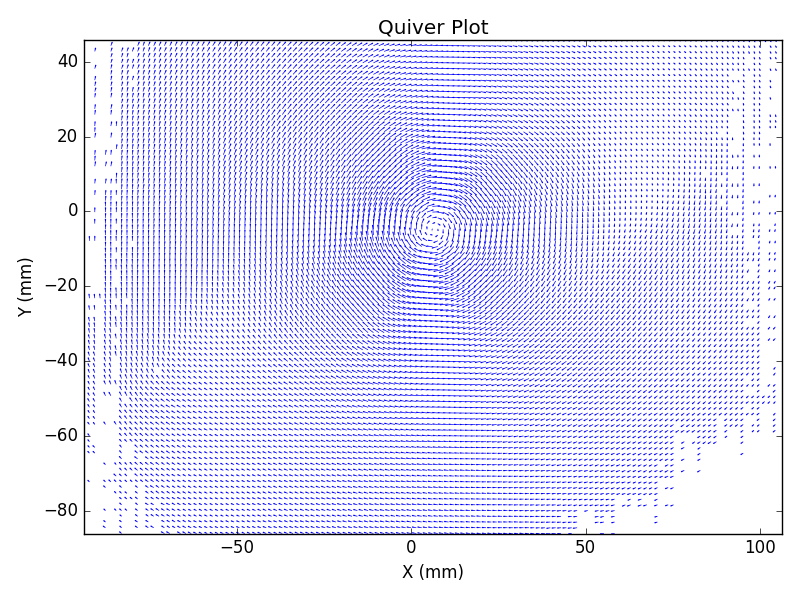
\includegraphics[width=5in]{figs/example_vortex_figs/example_quiver}
	\caption{Velocity vector field of a vortical flow structure as produced by 
	PIV.}
	\label{fig:quiver_example}
\end{figure}

 
\subsection{The Case for PIV}

Unlike other flow measurement techniques, PIV is a non-invasive method to 
directly measure time and displacement, and thus velocity. PIV is also capable 
of resolving vector measurements at many positions within a two dimensional 
slice of the flow field simultaneously, while other measurement techniques 
require taking data at many locations sequentially over a much greater period 
of time. PIV measurements can also be used to infer lift and drag forces on an 
solid body \cite{noca1997}. Single camera PIV can measure two components of the 
velocity vectors aligned with the image plane, but the PIV method is capable of 
resolving many dimensions of fluid flow with incremental increases in system 
complexity. The addition of another camera allows the full three dimensional 
velocity vector to be measured, and a sweeping beam laser or holographic PIV 
architecture allows the interrogation of an entire volume of flow field instead 
of a slice \cite{barnhart1994,elsinga2006,kahler2000}.

Stereo PIV is used widely because it provides a full velocity vector, and 
requires only an additional camera, slightly more complex calibration and 
software to process the imagery. A stereo PIV system with a 
stationary sheet laser can resolve three dimensional velocity vectors and their 
fluctuations within a two dimensional slice of fluid flow. A two point 
correlation tensor containing important information about the turbulent 
structure of a flow can be obtained readily with PIV. The non-invasive nature 
of PIV, combined with the  ability to interrogate a flow volume very quickly 
for information with high dimensionality makes it exceptionally useful in fluid 
mechanics. \cite{adrian1991}

\subsubsection{PIV for the study of Turbulence}
The study of turbulent flows requires a large range of spatial and velocity 
scales. Therefore, measurement techniques used to study turbulent phenomena 
require a significant spread between the lowest measurable velocity, and the 
highest \cite{barnhart1994}. Though PIV has grown in popularity, it is not a 
complete replacement for more mature techniques including hot-wire anemometry. 
It has been shown that the attenuation of the velocity and velocity derivative 
statistics is significantly higher with PIV than with hot-wire anemometry due 
to the volume averaging associated with PIV techniques. 
However, correction procedures have been developed that allow corrected PIV 
measurements of turbulent kinetic energy to agree closely with hot-wire 
anemometry measurements \cite{lavoie2007,kasagi1991}. 

Reynolds stresses can be extracted from the two point correlation averaged over 
an interrogation window. With this technique, one Reynolds stress value will be 
obtained for each of the smallest interrogation windows, which are typically 
several pixels in size. In this technique, the particle displacements are found 
by finding the peak of the correlation function of image pairs, transformed 
into velocities and broken down into stable and fluctuating components typical 
of a Reynolds averaging approach. Alternatively, single-pixel resolution 
Reynolds stress measurements can be obtained by direct examination of the 
correlation function. This technique can estimate Reynolds stresses at an 
enhanced resolution with a few percentage points of error with a set of several 
thousand PIV image pairs \cite{scharnowski2011}.

\subsection{Principles of Planar PIV}

A simple planar PIV system consists of a double pulsed laser, light sheet 
forming optics, particle seed, a single lens camera, image digitization 
hardware, and a computer system for data storage and subsequent analysis. The 
optical geometry of a planar PIV experiment is shown in figure 
\ref{fig:mono_piv}.

\begin{figure}[H]
	\centering
	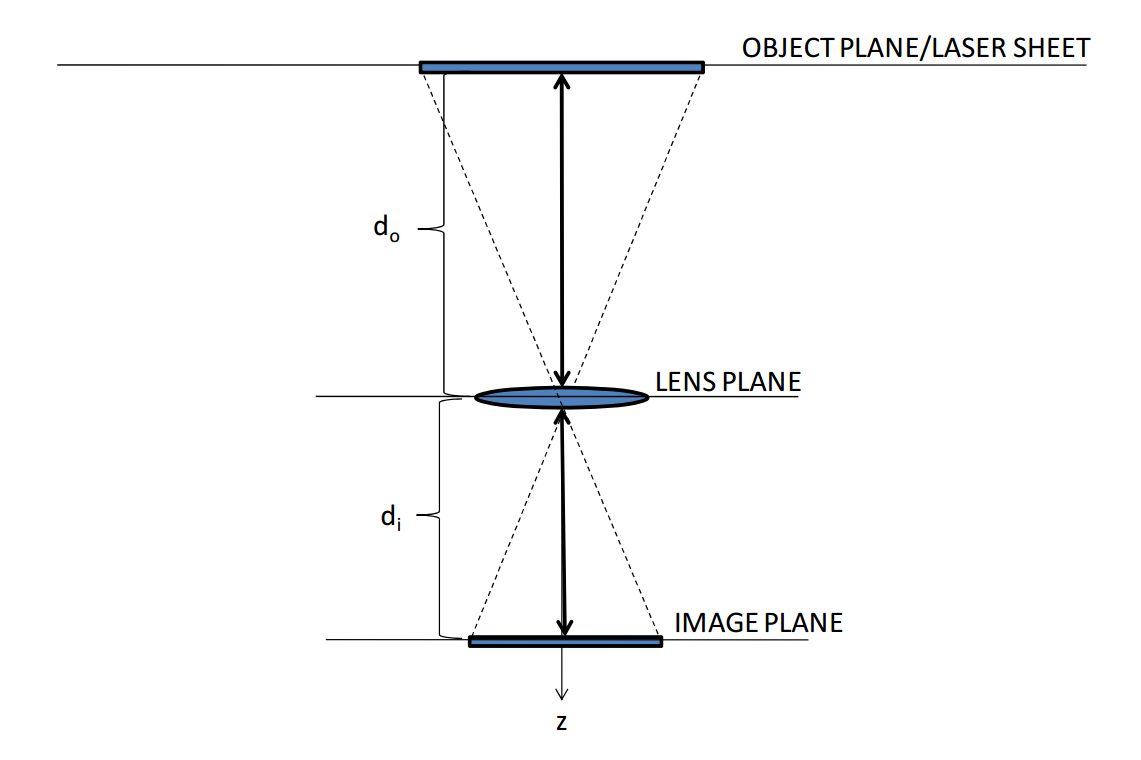
\includegraphics[width=5in]{figs/piv_method/mono_piv_optics}
	\caption{Single camera PIV system for mapping two dimensional velocity 
		vectors}
	\label{fig:mono_piv}
\end{figure} 

The 
underlying concept behind all PIV is that light scattered from the particles as 
they move through the flow field allows a pair of images to capture information 
about the motion of that particle. Double pulsed illumination is commonly used 
in PIV systems due to its relatively low cost and complexity compared with 
multiple laser source systems. The energy required to adequately illuminate an 
area of interest depends upon the size of that area, and the scattering 
properties of the particle seed. Solid state Nd:YAG lasers are typically used 
for this purpose \cite{adrian2011}. An $(X, Y, Z)$ coordinate system 
is defined 
within the light sheet that exists in $(X, Y)$ space, and relates linearly to a 
coordinate system in the image plane of the camera in $(X_p, Y_p)$ pixel space. 
At a time $t$, a laser light sheet is produced for a short pulse and the camera 
captures an image of the light scattering from particles within the flow. At 
some short time later, $t + dt$, a second pulse occurs and a second image is 
taken. By measuring the pixel displacements $(\Delta X_p, \Delta 
Y_p)$ for a particle in the image plane, and transforming the coordinates into 
the plane of the laser one obtains $(\Delta X, \Delta Y, \Delta Z)$. This 
coordinate transform can be obtained from precise information about the optical 
geometry of the system, or by direct measurement of calibration data 
\cite{fouras2007}.The method of direct measurement of a calibration target was 
used in this research. 

The detection rate, accuracy, and reliability of PIV depends upon careful 
selection of experimental parameters. Kean and Adrian suggest a set of six 
important dimensionless quantities and ideal operating ranges that improve the 
chances of high quality PIV results . The parameters 
are data validation criterion, particle image density, relative in-plane image 
displacement, relative out-of-plane displacement, velocity gradient, and the 
ratio of the mean image diameter to the interrogation spot diameter 
\cite{keane1990,lawson1997b}. Steep velocity gradients create random 
errors as the 
individual particle displacements cover a discreet range within an 
interrogation spot. Particle displacements should be restricted to 25\% of the 
interrogation spot diameter for in-plane velocities, and to 25\% of the light 
sheet thickness in out-of-plane velocities. One way to mitigate both of these 
effects is to use as high resolution PIV as possible, or by scaling the 
interrogation area down by altering the zoom of the cameras. Since the velocity 
profile of an axial vortex can contain high velocity gradients in the vicinity 
of the core, and both in-plane and out-of-plane velocities are expected to be 
high, the present experiments used 50mm lenses to zoom each camera to 
focus on a small an interrogation plane as possible \cite{prasad1992}.

\subsection{Principles of Stereo PIV}

Classical single camera PIV is only capable of capturing the projection of the 
velocity vector on the image plane. The out-of-plane component is lost 
completely, and the in-plane components are affected by unrecoverable error. In 
Stereo PIV, a pair of cameras may obliquely view the same plane and the entire 
3d velocity vector may be inferred using the camera geometry. This technique 
includes tilting the backplanes of the cameras to satisfy the Scheimpflug image 
criteria and a dewarping function based on camera geometry to account for 
projective distortion \cite{willert1997}. An example of the geometric set up 
used by Willert to study the movement of a ring vortex through the 
interrogation plane is shown in Figure \ref{fig:stereo_piv}. Uncertainties 
associated with high out-of-plane motion in planar PIV are greatly reduced in 
stereo PIV \cite{lawson1997b,lawson1997}.

\begin{figure}[H]
	\centering
	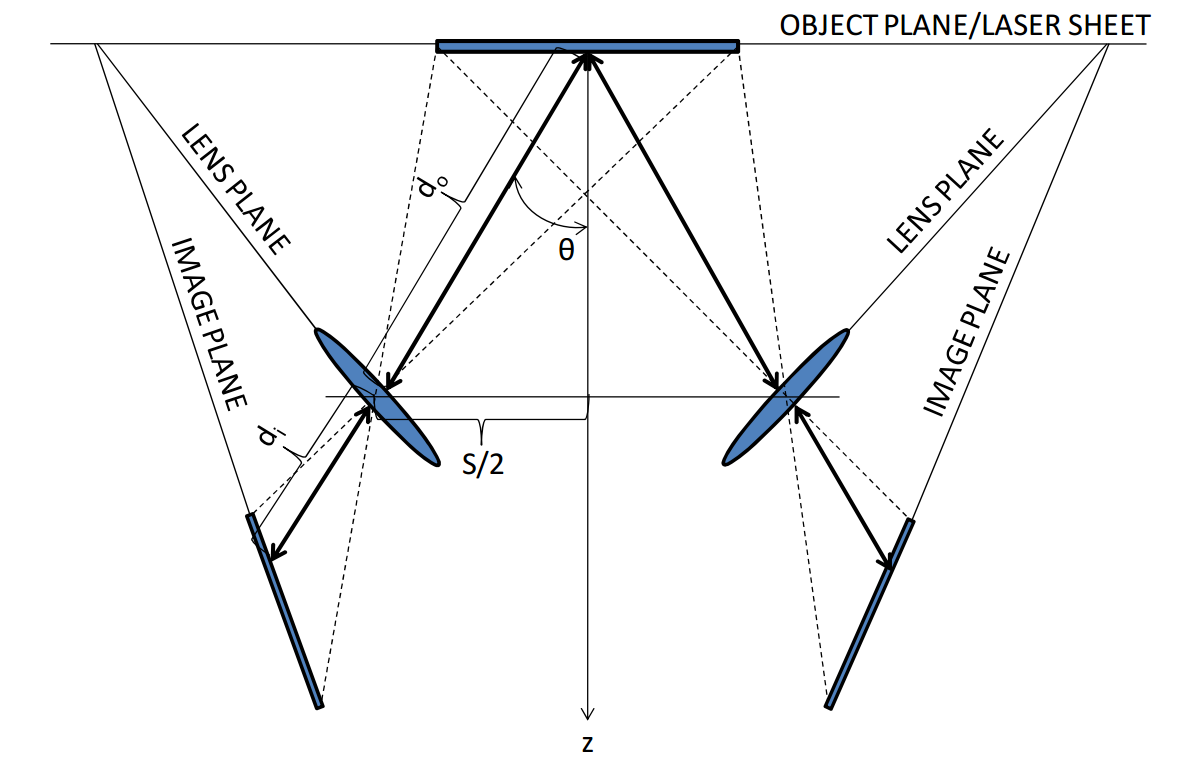
\includegraphics[width=5in]{figs/piv_method/stereo_piv_optics}
	\caption{Stereo camera PIV system for mapping three dimensional velocity 
		vectors}
	\label{fig:stereo_piv}
\end{figure}  

\subsection{Particles}

The "Particles" part of the PIV acronym refers to the small, highly reflective 
solid or liquid spheres that are entrained within a flow. It is assumed that 
the movement of the particles is representative of the fluid which propels them 
through the air, but this assumption deserves further examination 
\cite{roscoe1952}. Since particles have mass and inertia, the particles motion 
is a function of the force exerted upon it by the fluid, and by gravitational 
or magnetic body forces. As a particle travels along and encounters fluid which 
has changed direction, it does not respond instantaneously. The particles exact 
response to rapid changes in velocity in the carrying fluid is of great 
interest to the study of turbulence. It has been found that lightweight 
particles have a tendency to collect in regions of high strain rate and low 
vorticity. However, extremely light particles exhibit weaker preferential 
concentration as they more accurately follow fluid motion, and very heavy 
particles are relatively insensitive to turbulent velocity fluctuations 
\cite{squires1990}. Evidence of preferential particle collection can be seen in 
wake vortex PIV, as the vortex core is identifiable as a small spot of lower 
particle density as in figure \ref{fig:vortex_core_particles}.
	
\begin{figure}
	\centering
	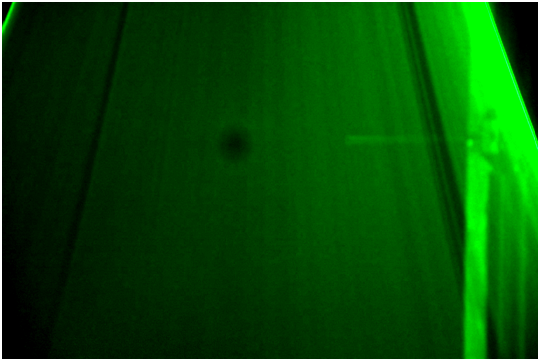
\includegraphics[width=4in]{figs/piv_method/vortex_core}
	\caption{Contrast enhanced image of an illuminated cross section showing a 
	low particle density in the vortex core.}
	\label{fig:vortex_core_particles}
\end{figure}

As a particles inertia and diameter shrinks, it becomes capable of following 
smaller turbulent length scales, but the prime consideration for particles is 
the ability to detect them. The intensity of the light reflecting from a 
particles should be sufficient to reach 30\% to 50\% of the saturation level of 
the recording medium. The controlling factors for intensity of reflected light 
are particle size, laser power, and refractive index \cite{adrian2011}. Thus, 
particles which are small enough to ensure turbulent structures on the time and 
length scales of interest can be adequately represented in the particles 
motion, but large enough to be detected must be selected. It has been 
demonstrated that particles on the scale of one micrometer and between 0.56 and 
1.62 times the density of the fluid, the particles can accurately represent 
turbulent structures on the order of many thousand Hertz \cite{mei1996}. In the 
present study, $CO_2$ filled mineral oil bubbles generated with a Laskin 
nozzle fog generater were used as particle seed. These droplets have a nominal 
diameter of 0.6 micrometers and densities of 1.55 times that of air were used.

The density of particle seeding must be sufficient for a correlation to be 
generated between frames for every small interrogation spot in the survey 
plane. In an instance where only one or two particles are visible in the first 
frame at the edge of an interrogation sector, then those particles exit the 
sector for the second frame, to be replaced by new particles 
entering the area from the other side, spurious results will be produced. 
Excessively dense particles 


\subsection{Image processing}

There are multiple methods for extracting vector fields from images of 
particles. A commonality between all methods is the use of a correlation 
function to find particle displacements. The correlation map is computed by 
taking the inverse fast Fourier transform (FFT) of the product of the FFT of 
the first image, and the complex conjugate of the FFT of the second image, then 
adjusting for up-sampling by dividing by the original factor as in equation. 
Displacement is measured by finding the peak of correlation map between a small 
sector of each image, represented by Equation \ref{eq:correlation_map}. 

\begin{equation}
C_{map} = FFT^{-1} * [F_A \times conj(F_B) ]
\label{eq:correlation_map}
\end{equation}

where $C_{map}$ is the correlation map, $F_A$ is the fast Fourier transform of 
image $A$, at time $t=0$ and $F_B$ is the fast Fourier transform of image $B$ 
at time $t=dt$. This process is repeated many times to create a vector field of 
pixel displacements. In the simplest case, these correlation maps are 
considered individually, and the absolute highest peak is used to determine the 
mean pixel displacement within a sector. The Hart method, which was used in the 
present study, improves upon this with element by element comparison of 
adjacent sectors correlation tables to remove false peaks 
\cite{hart1998,hart1999}.

The mathematics behind derivation of velocity vector fields from stereo image 
pairs is based upon coordinate transformations from pixel coordinates to real 
coordinates with the following Equations 
\ref{eq:piv_to_real1} to \ref{eq:piv_to_real4}.

\begin{equation}
x_L= X\frac{dx_L}{dX} + Y\frac{dx_L}{dY} + Z\frac{dx_L}{dZ}
\label{eq:piv_to_real1}
\end{equation}

\begin{equation}
x_R= X\frac{dx_R}{dX} + Y\frac{dx_R}{dY} + Z\frac{dx_R}{dZ}
\label{eq:piv_to_real2}
\end{equation}

\begin{equation}
y_L= X\frac{dy_L}{dX} + Y\frac{dy_L}{dY} + Z\frac{dy_L}{dZ}
\label{eq:piv_to_real3}
\end{equation}

\begin{equation}
y_R= X\frac{dy_R}{dX} + Y\frac{dy_R}{dY} + Z\frac{dy_R}{dZ}
\label{eq:piv_to_real4}
\end{equation}

where $x_L$, $x_R$, $y_L$ and $y_R$ are the pixel displacements in the x 
direction on the left and right cameras, and the y direction on the left and 
right cameras respectively. Symbols $X$, $Y$, and $Z$ are real spatial particle 
displacements in the interrogation plane. The set of twelve derivatives are 
pixel displacement sensitivity coefficients, which are determined by a 
calibration process which involves taking pictures of a matrix of bright dots 
with a known distance between each dot. Once all twelve calibration 
coefficients are known, the set of equations is actually over constrained, with 
four equations and only three unknowns, a least squared method will be used to 
map measurements form the image plane to the real plane. In the case of this 
study, INSIGHT software was used to generate this set of calibration 
coefficients.

The image is 
up sampled to higher resolution to allow sub-pixel displacements to be 
measured, thus preventing accuracy limitations associated with the physical 
dimensions of each pixel. The image is typically divided into grids 16 by 16 
pixels in size, with 50\% overlap with surrounding grids to ensure particles 
which started inside the sector at $t=0$, but begin to exit the sector at 
$t=dt$, are still identifiable.  


Figure \ref{fig:piv_sector_0up} shows a sample of two side by side images taken 
several microseconds, $dt$ apart without any up-sampling. Figure 
\ref{fig:piv_sector_overlay_fft_0up} shows a sample of the same two images 
layered on top of each other to show the apparent horizontal displacement 
between the two images. The two dimensional correlation map shows a clear peak 
down at four pixels in the $X$ direction and zero pixels in the $Y$ direction.


\begin{figure}[H]
	\begin{subfigure}{.49\textwidth}
		\centering
		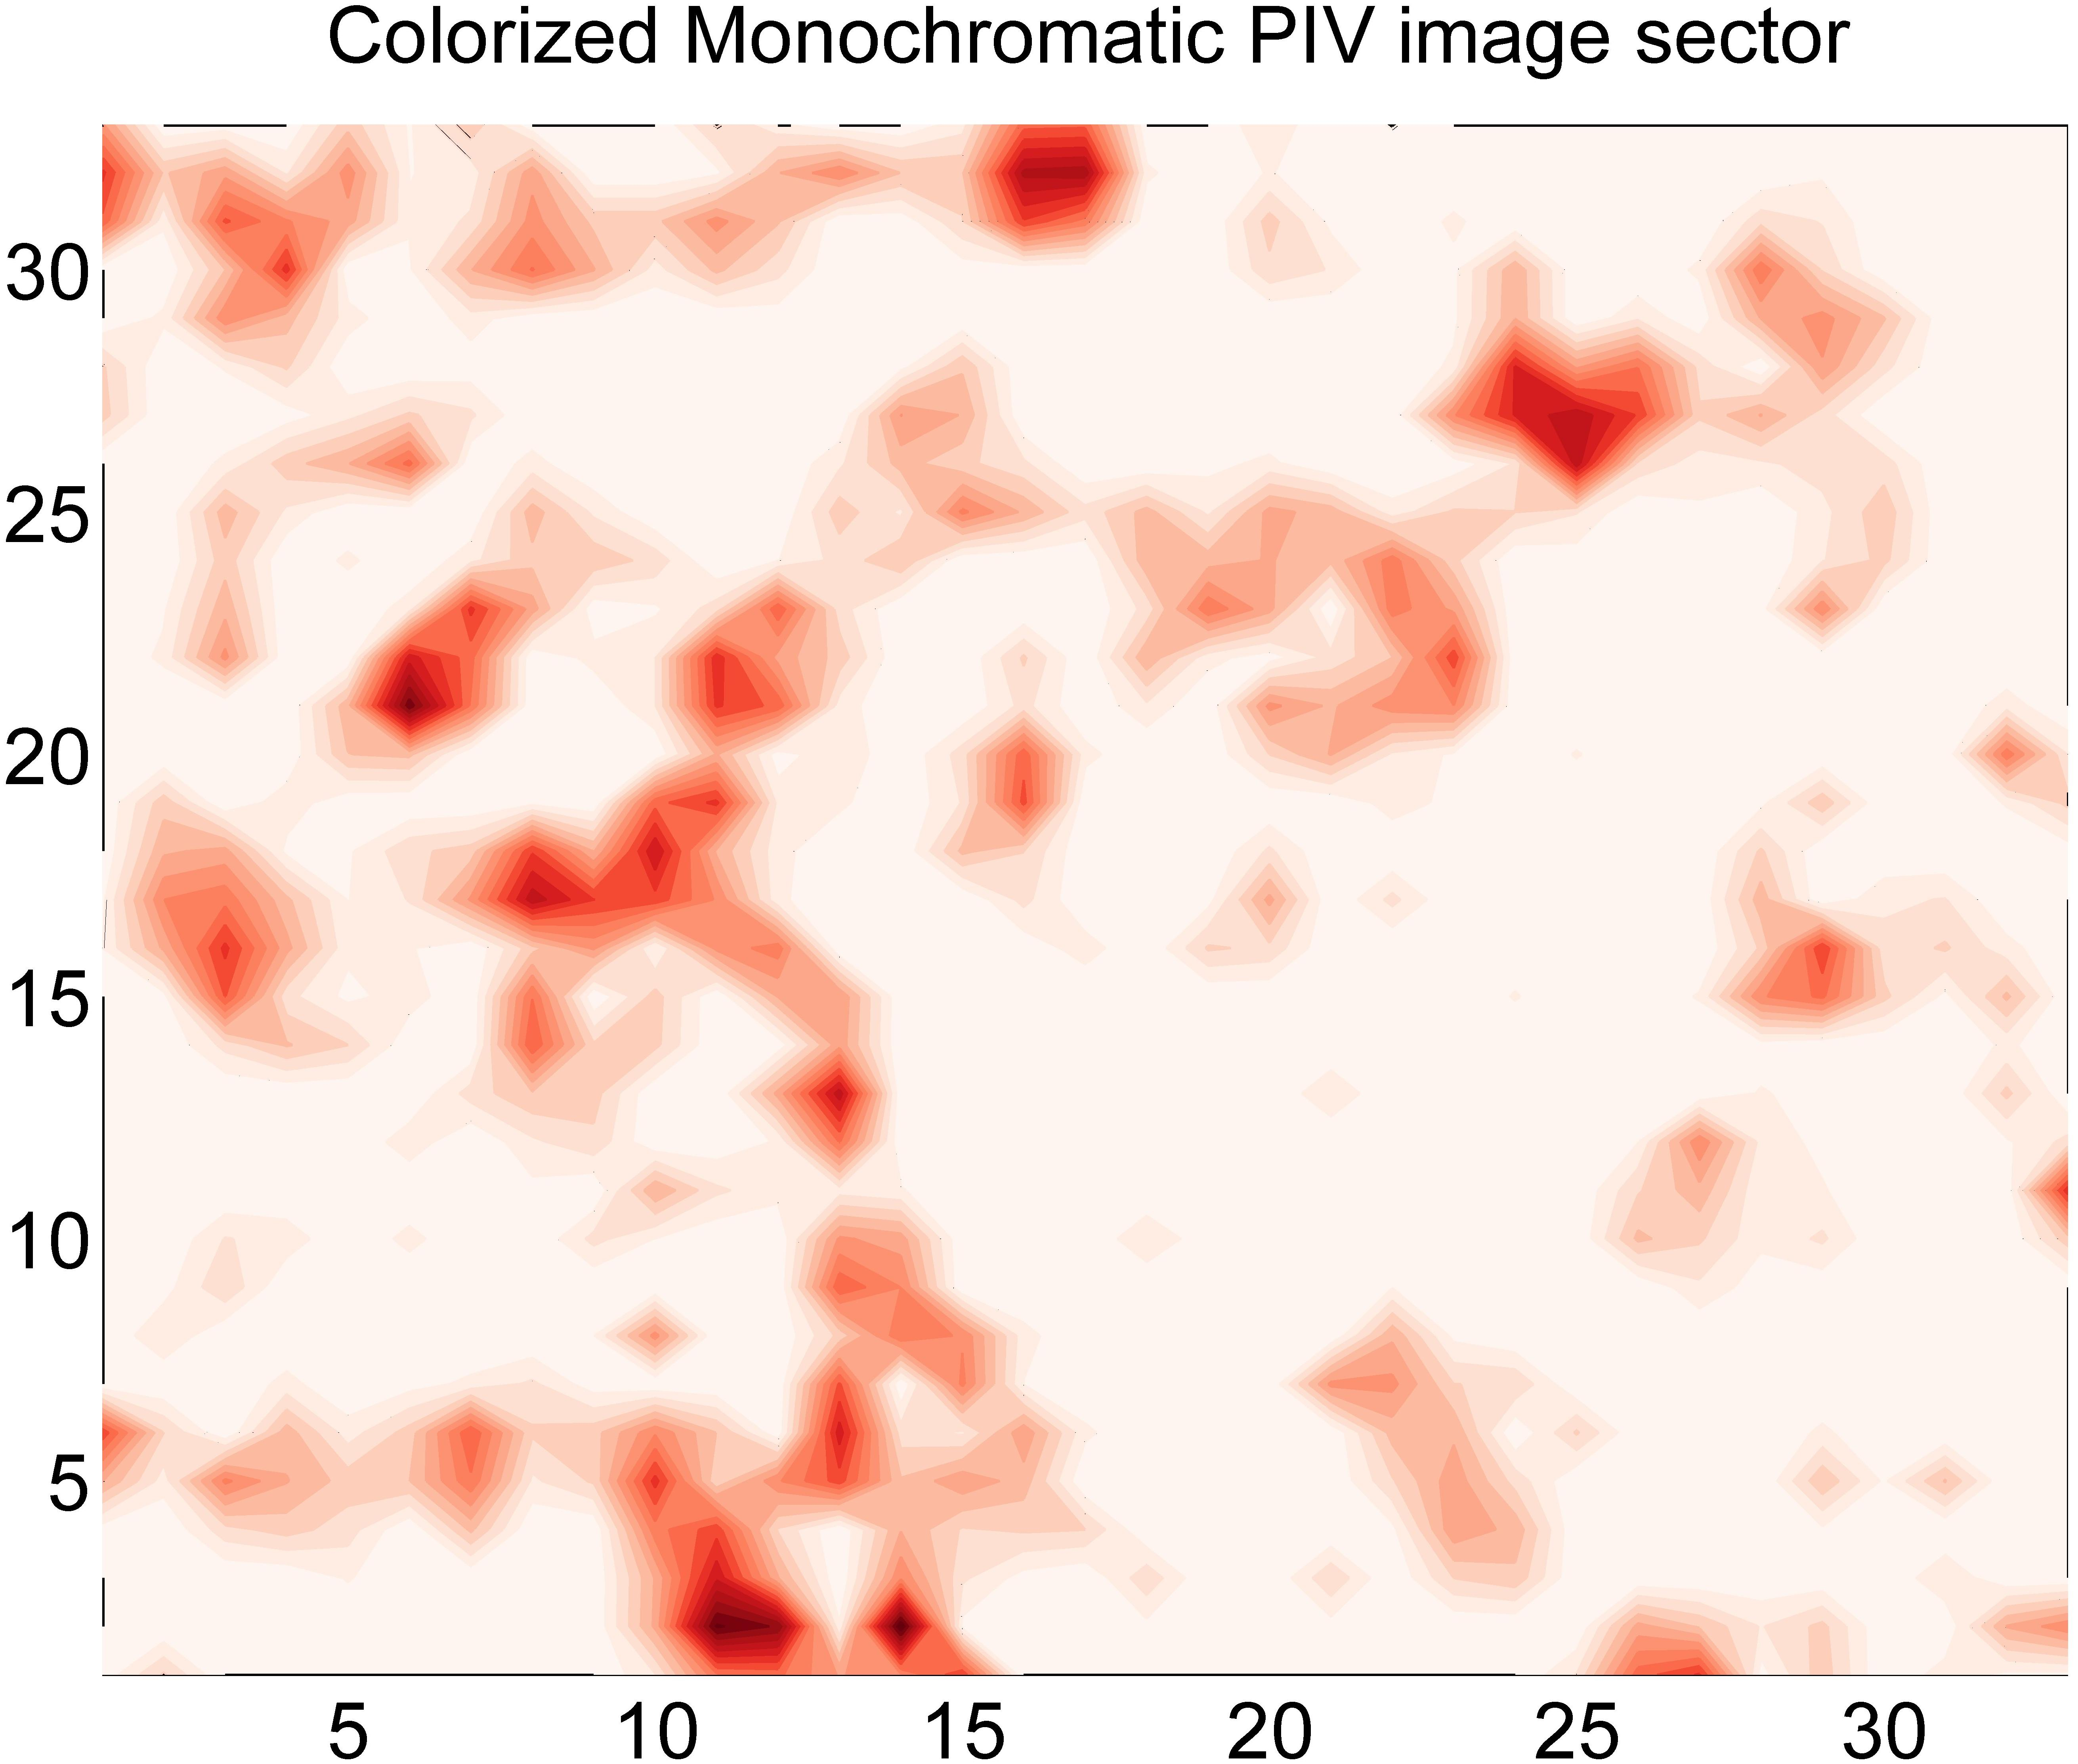
\includegraphics[width=.9\linewidth]{figs/piv_method/pive_figa_order0}
	\end{subfigure} 
	\begin{subfigure}{.49\textwidth}
		\centering
		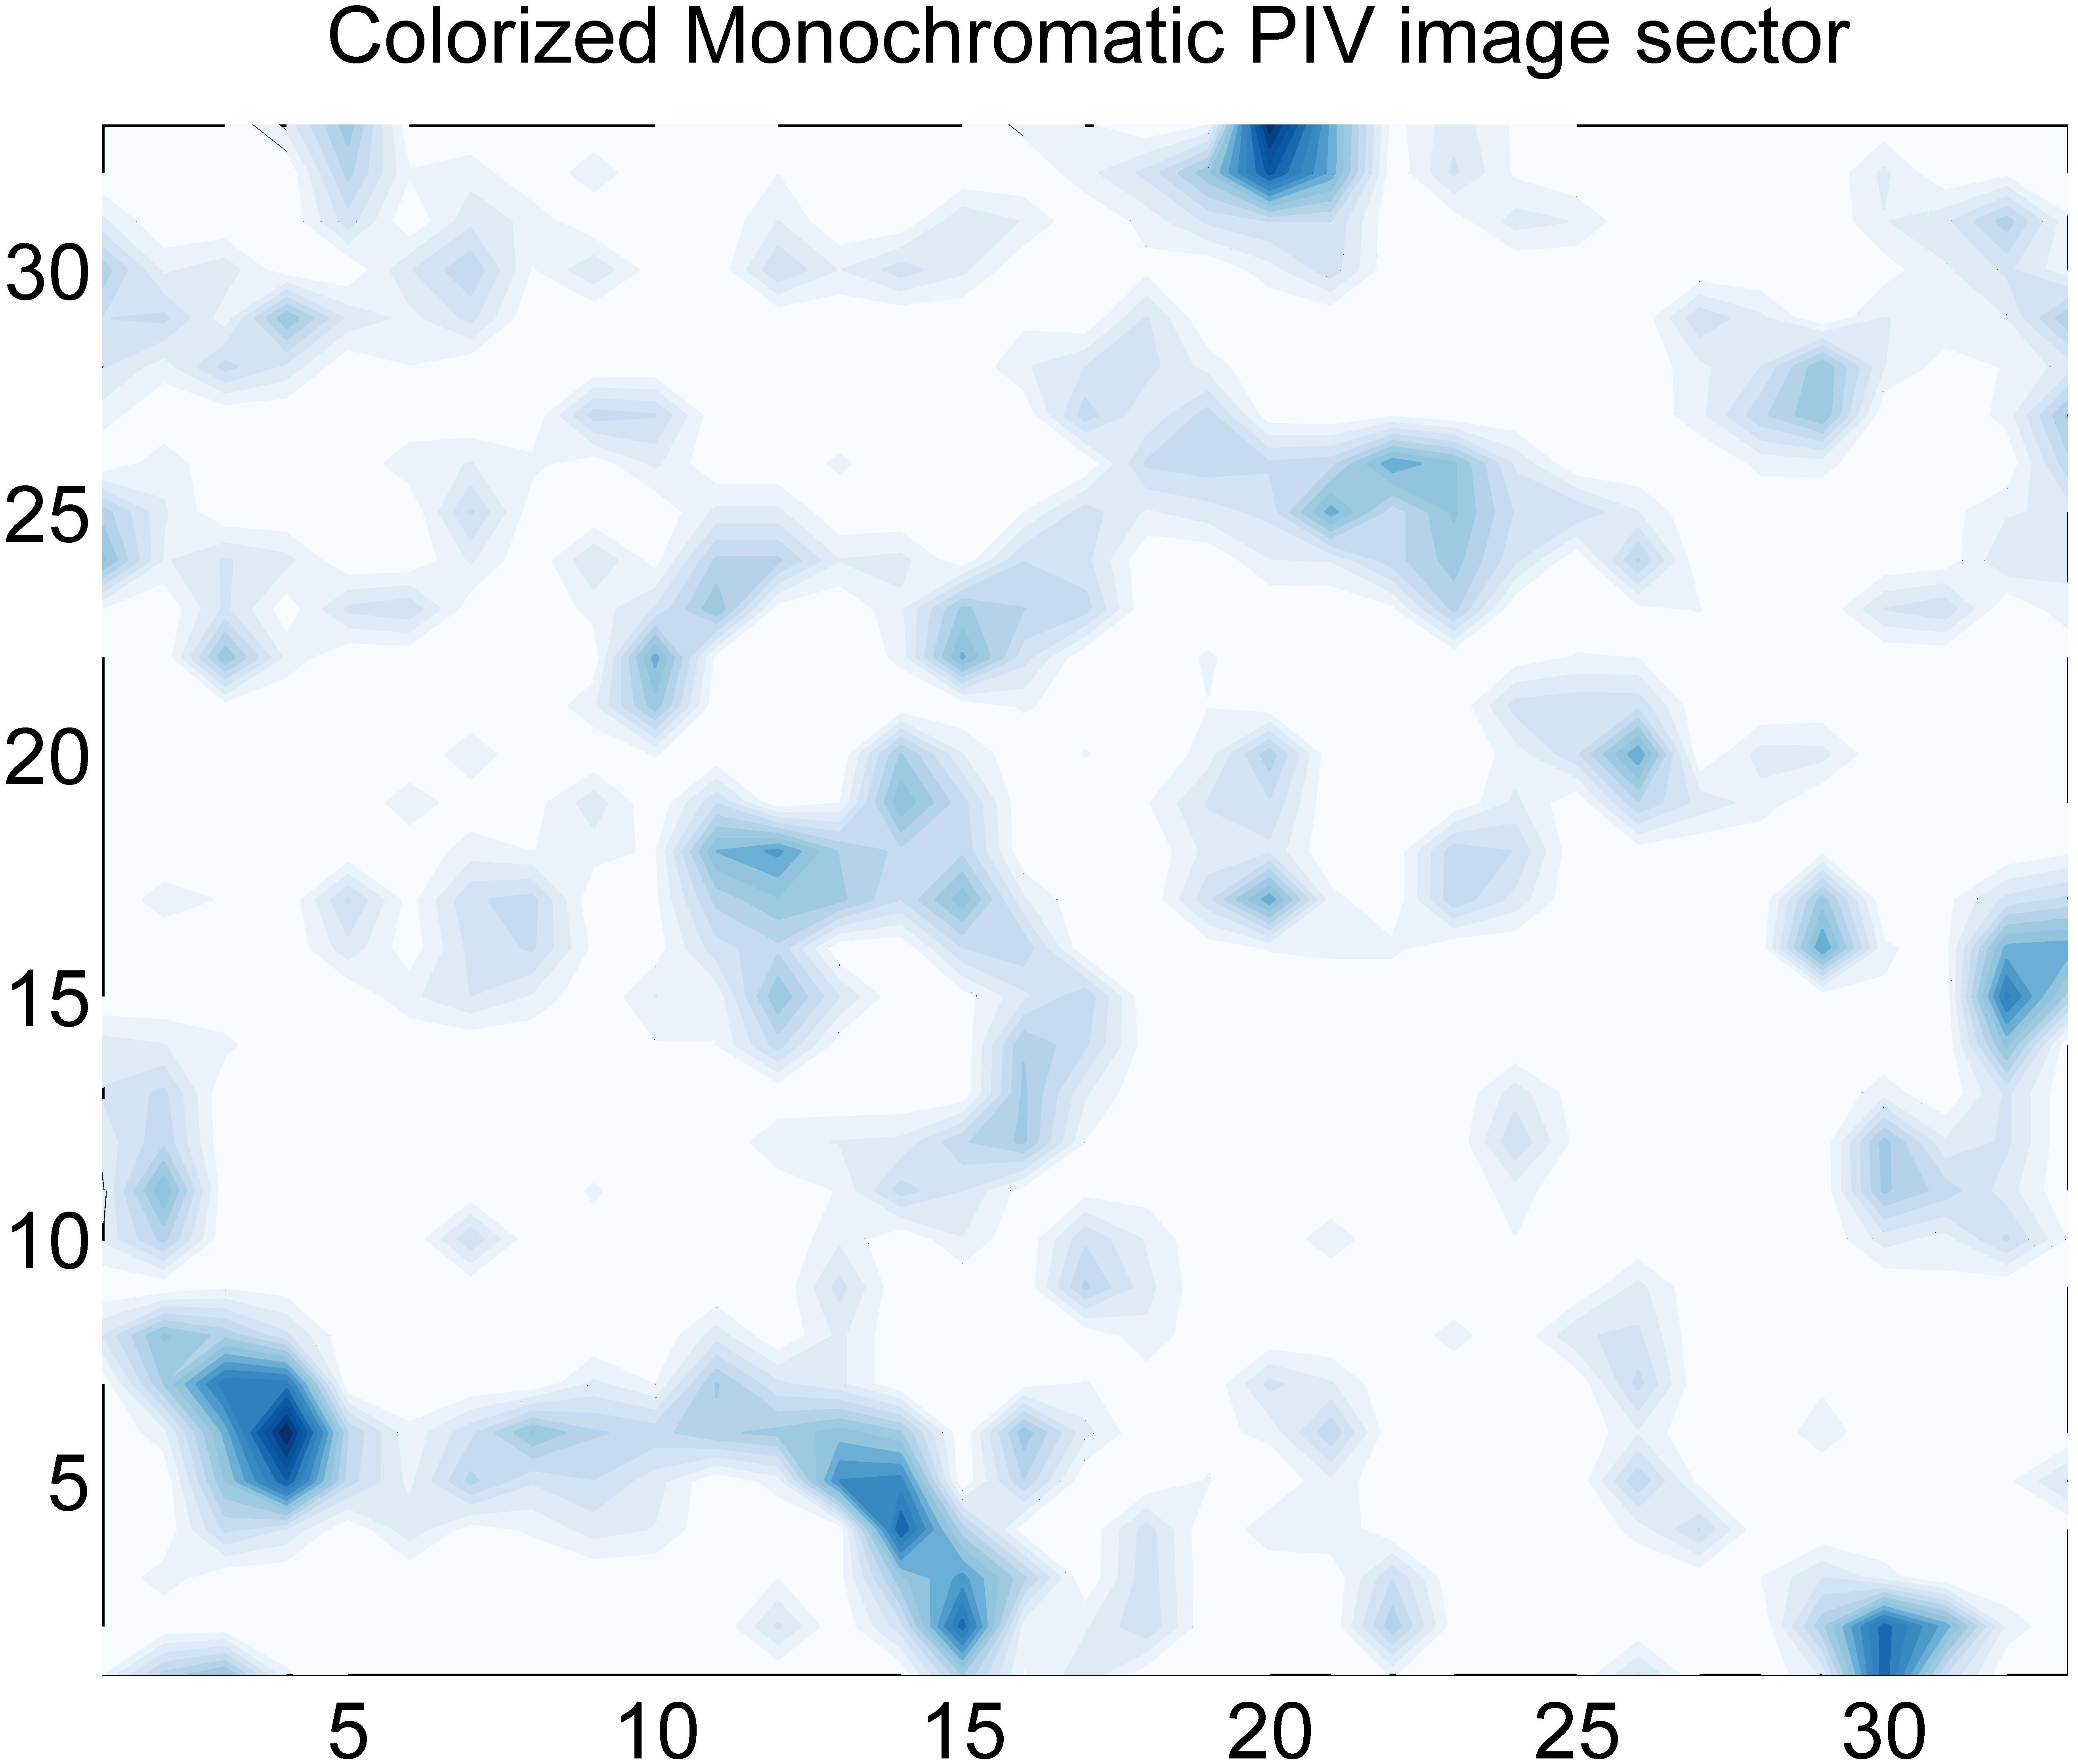
\includegraphics[width=.9\linewidth]{figs/piv_method/pive_figb_order0}
	\end{subfigure}	
	\caption{Colorized 32x32 pixel contour images at $t=0$ (left), and $t=dt$ 
		(right), no up sampling.}
	\label{fig:piv_sector_0up}
\end{figure}


\begin{figure}[H]
	\begin{subfigure}{.49\textwidth}
		\centering
		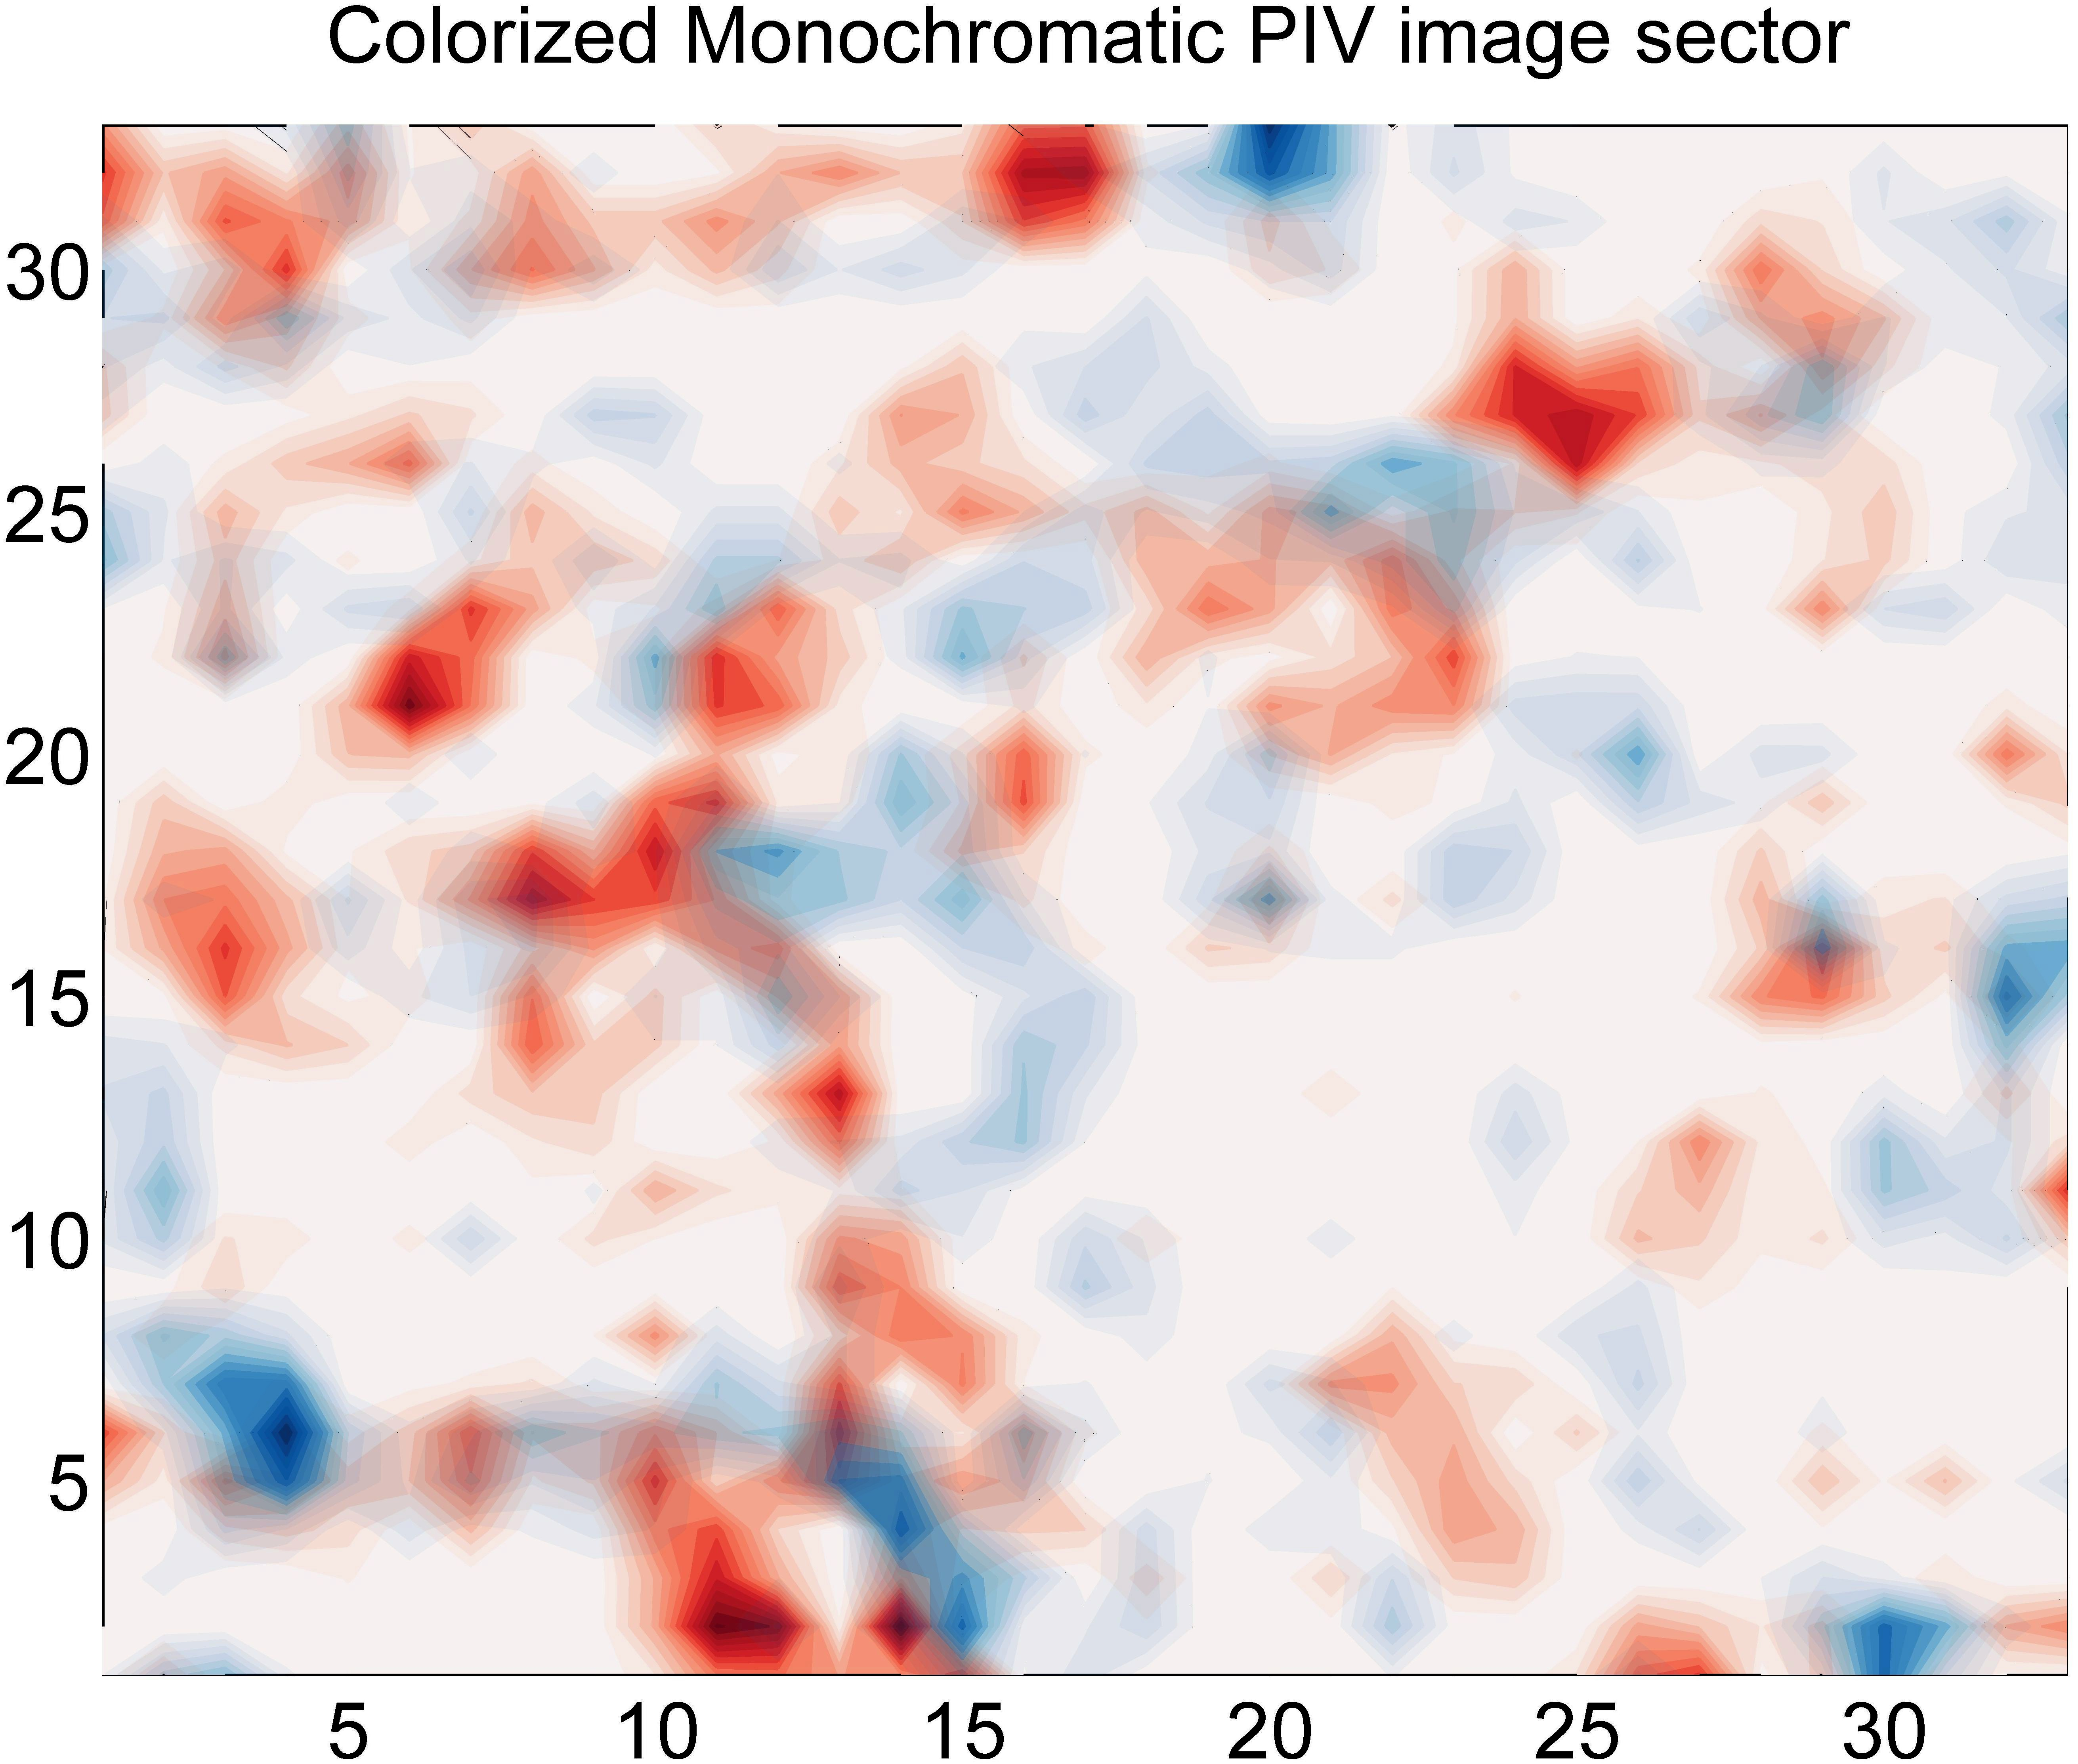
\includegraphics[width=.9\linewidth]{figs/piv_method/pive-fig_order0}
	\end{subfigure} 
	\begin{subfigure}{.49\textwidth}
		\centering
		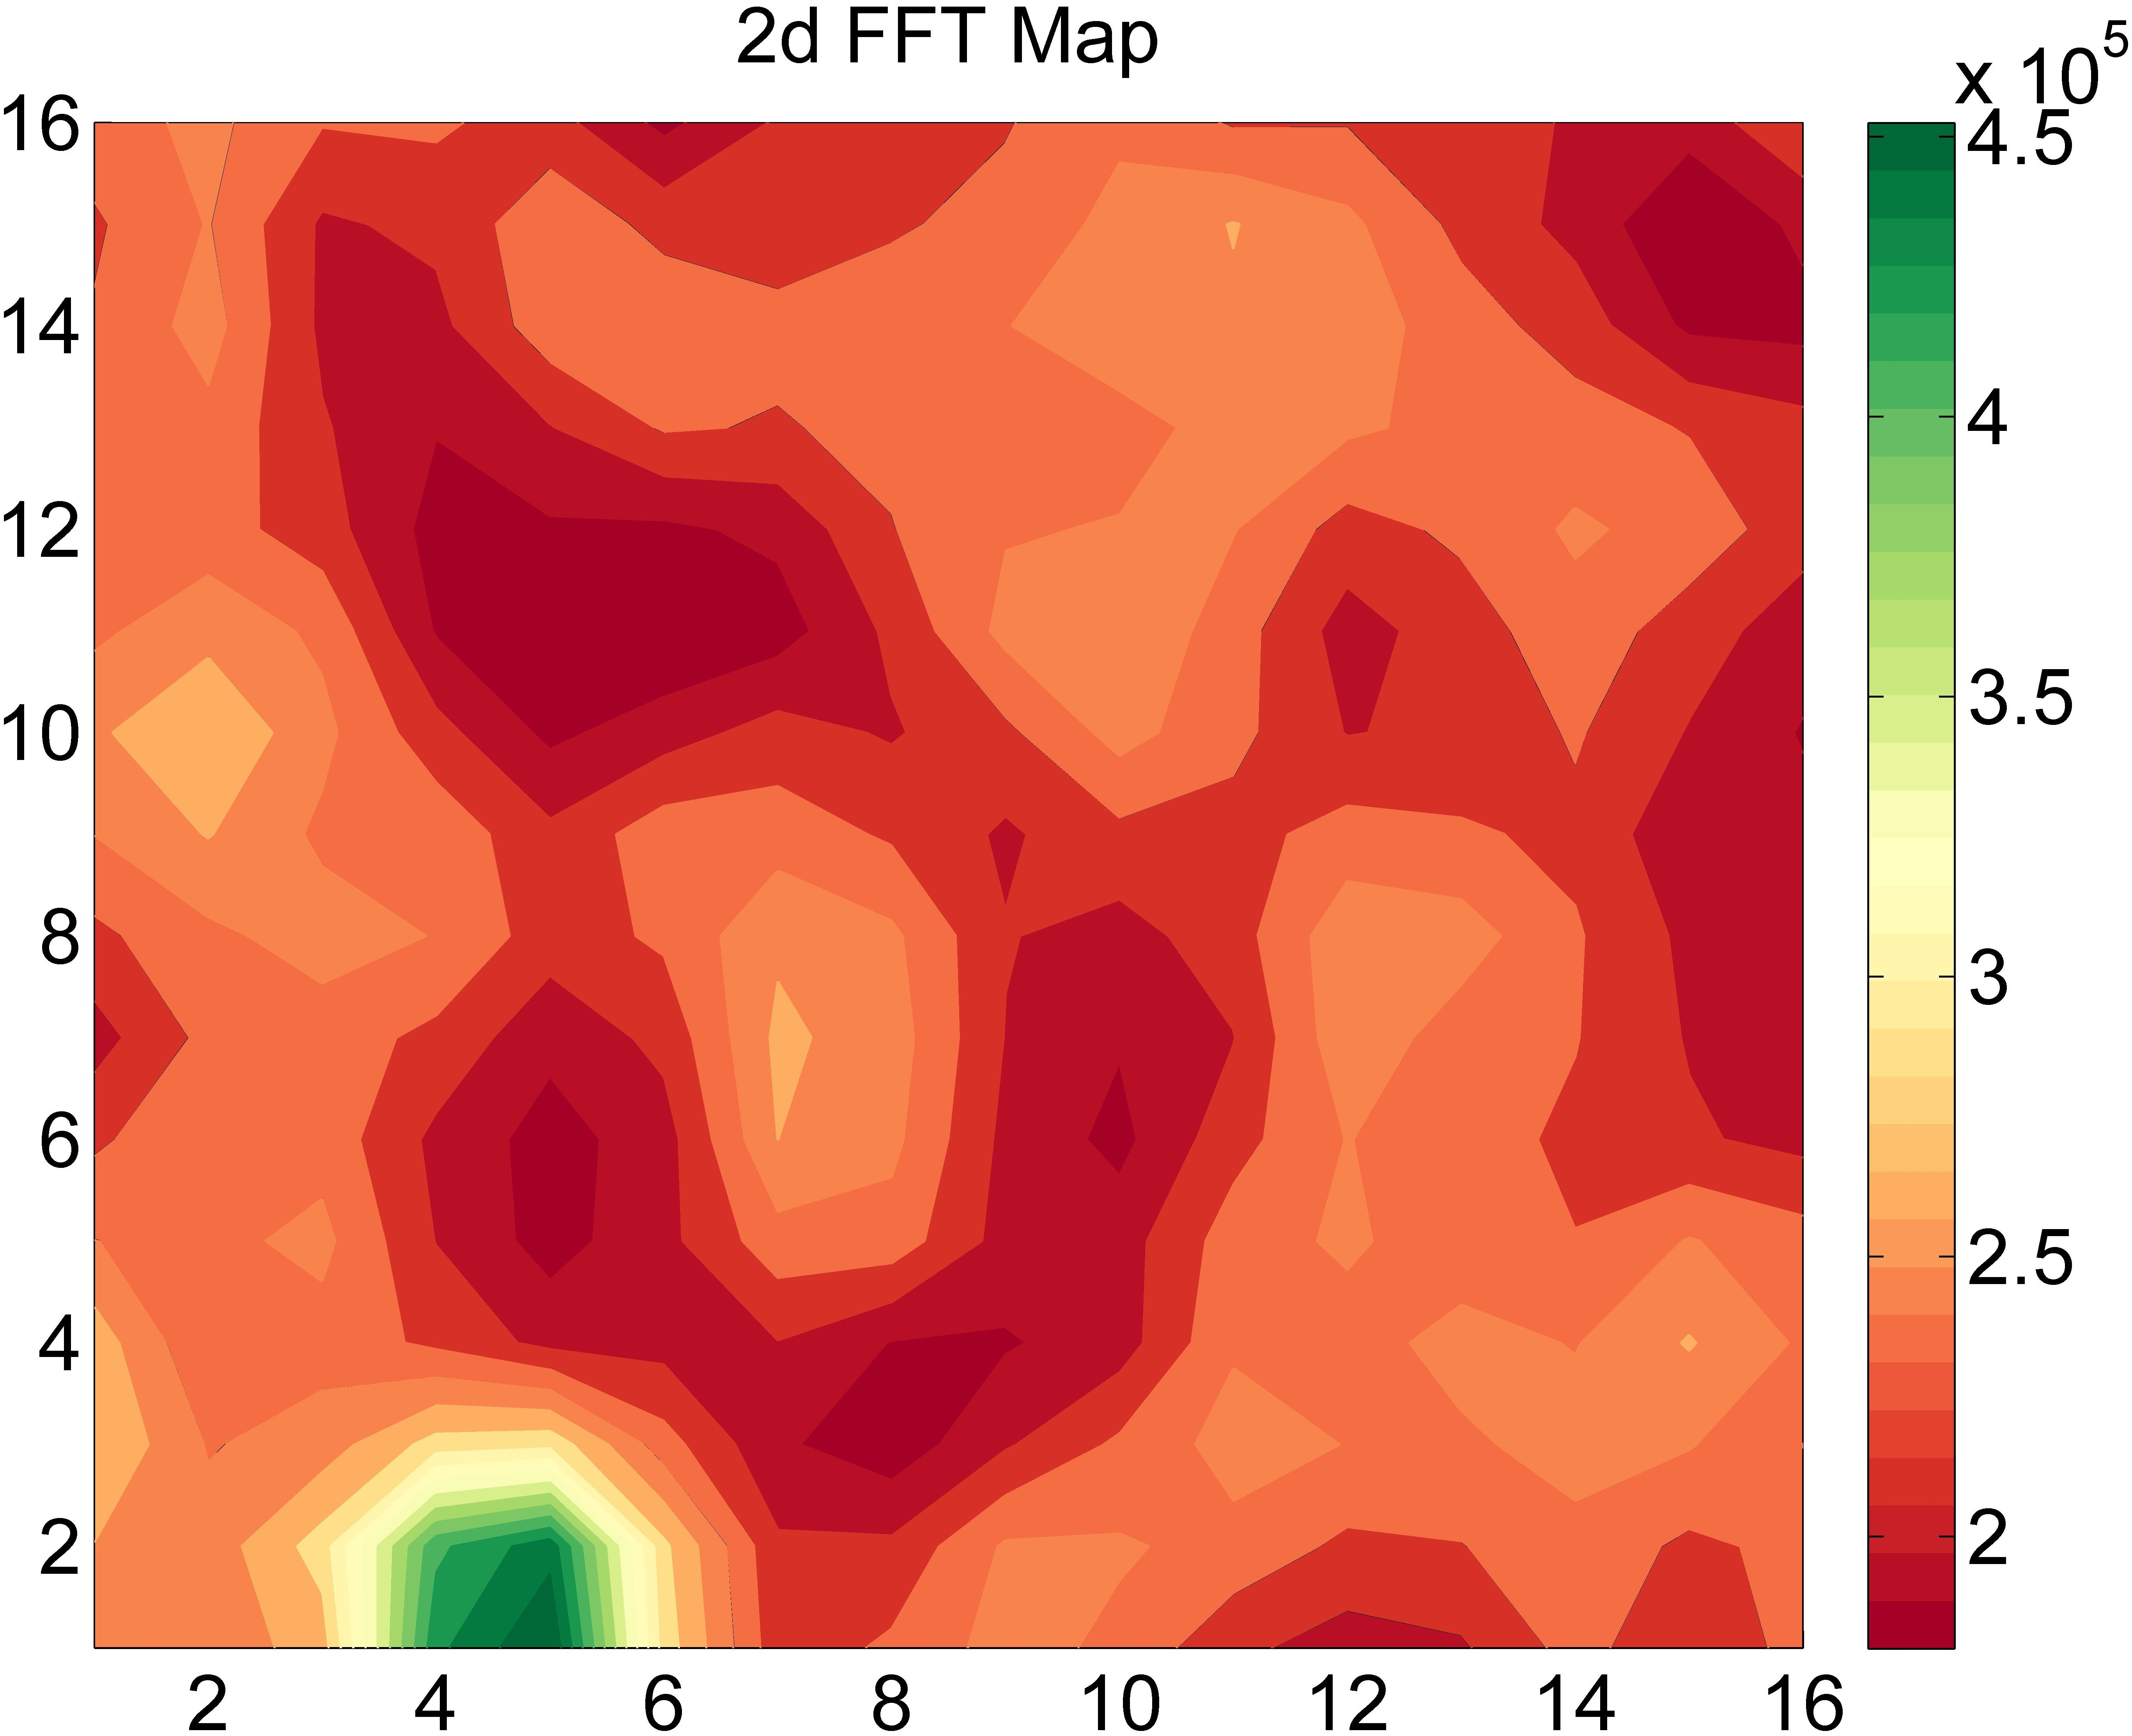
\includegraphics[width=.9\linewidth]{figs/piv_method/pive_fft_order0}
	\end{subfigure}	
	\caption{Overlaid sector snapshots (left) and corresponding correlation 
		map (right), no up sampling.}
	\label{fig:piv_sector_overlay_fft_0up}
\end{figure}


Every up sampling doubles the dimensions of the sector, quadrupling the number 
of pixels and increasing the sub-pixel resolution by a factor of two. The same 
set of figures is repeated for the same image with 6th order bilinear up 
sampling in figures \ref{fig:piv_sector_6up} and
\ref{fig:piv_sector_overlay_fft_6up}. Note that the images are much smoother, 
and the images have been sampled sufficiently to make a very finely spaced grid.
It is important to note that while bilinear up sampling is used for this
example, any other two dimensional method such as cubic may be used.

\begin{figure}[H]
	\begin{subfigure}{.49\textwidth}
		\centering
		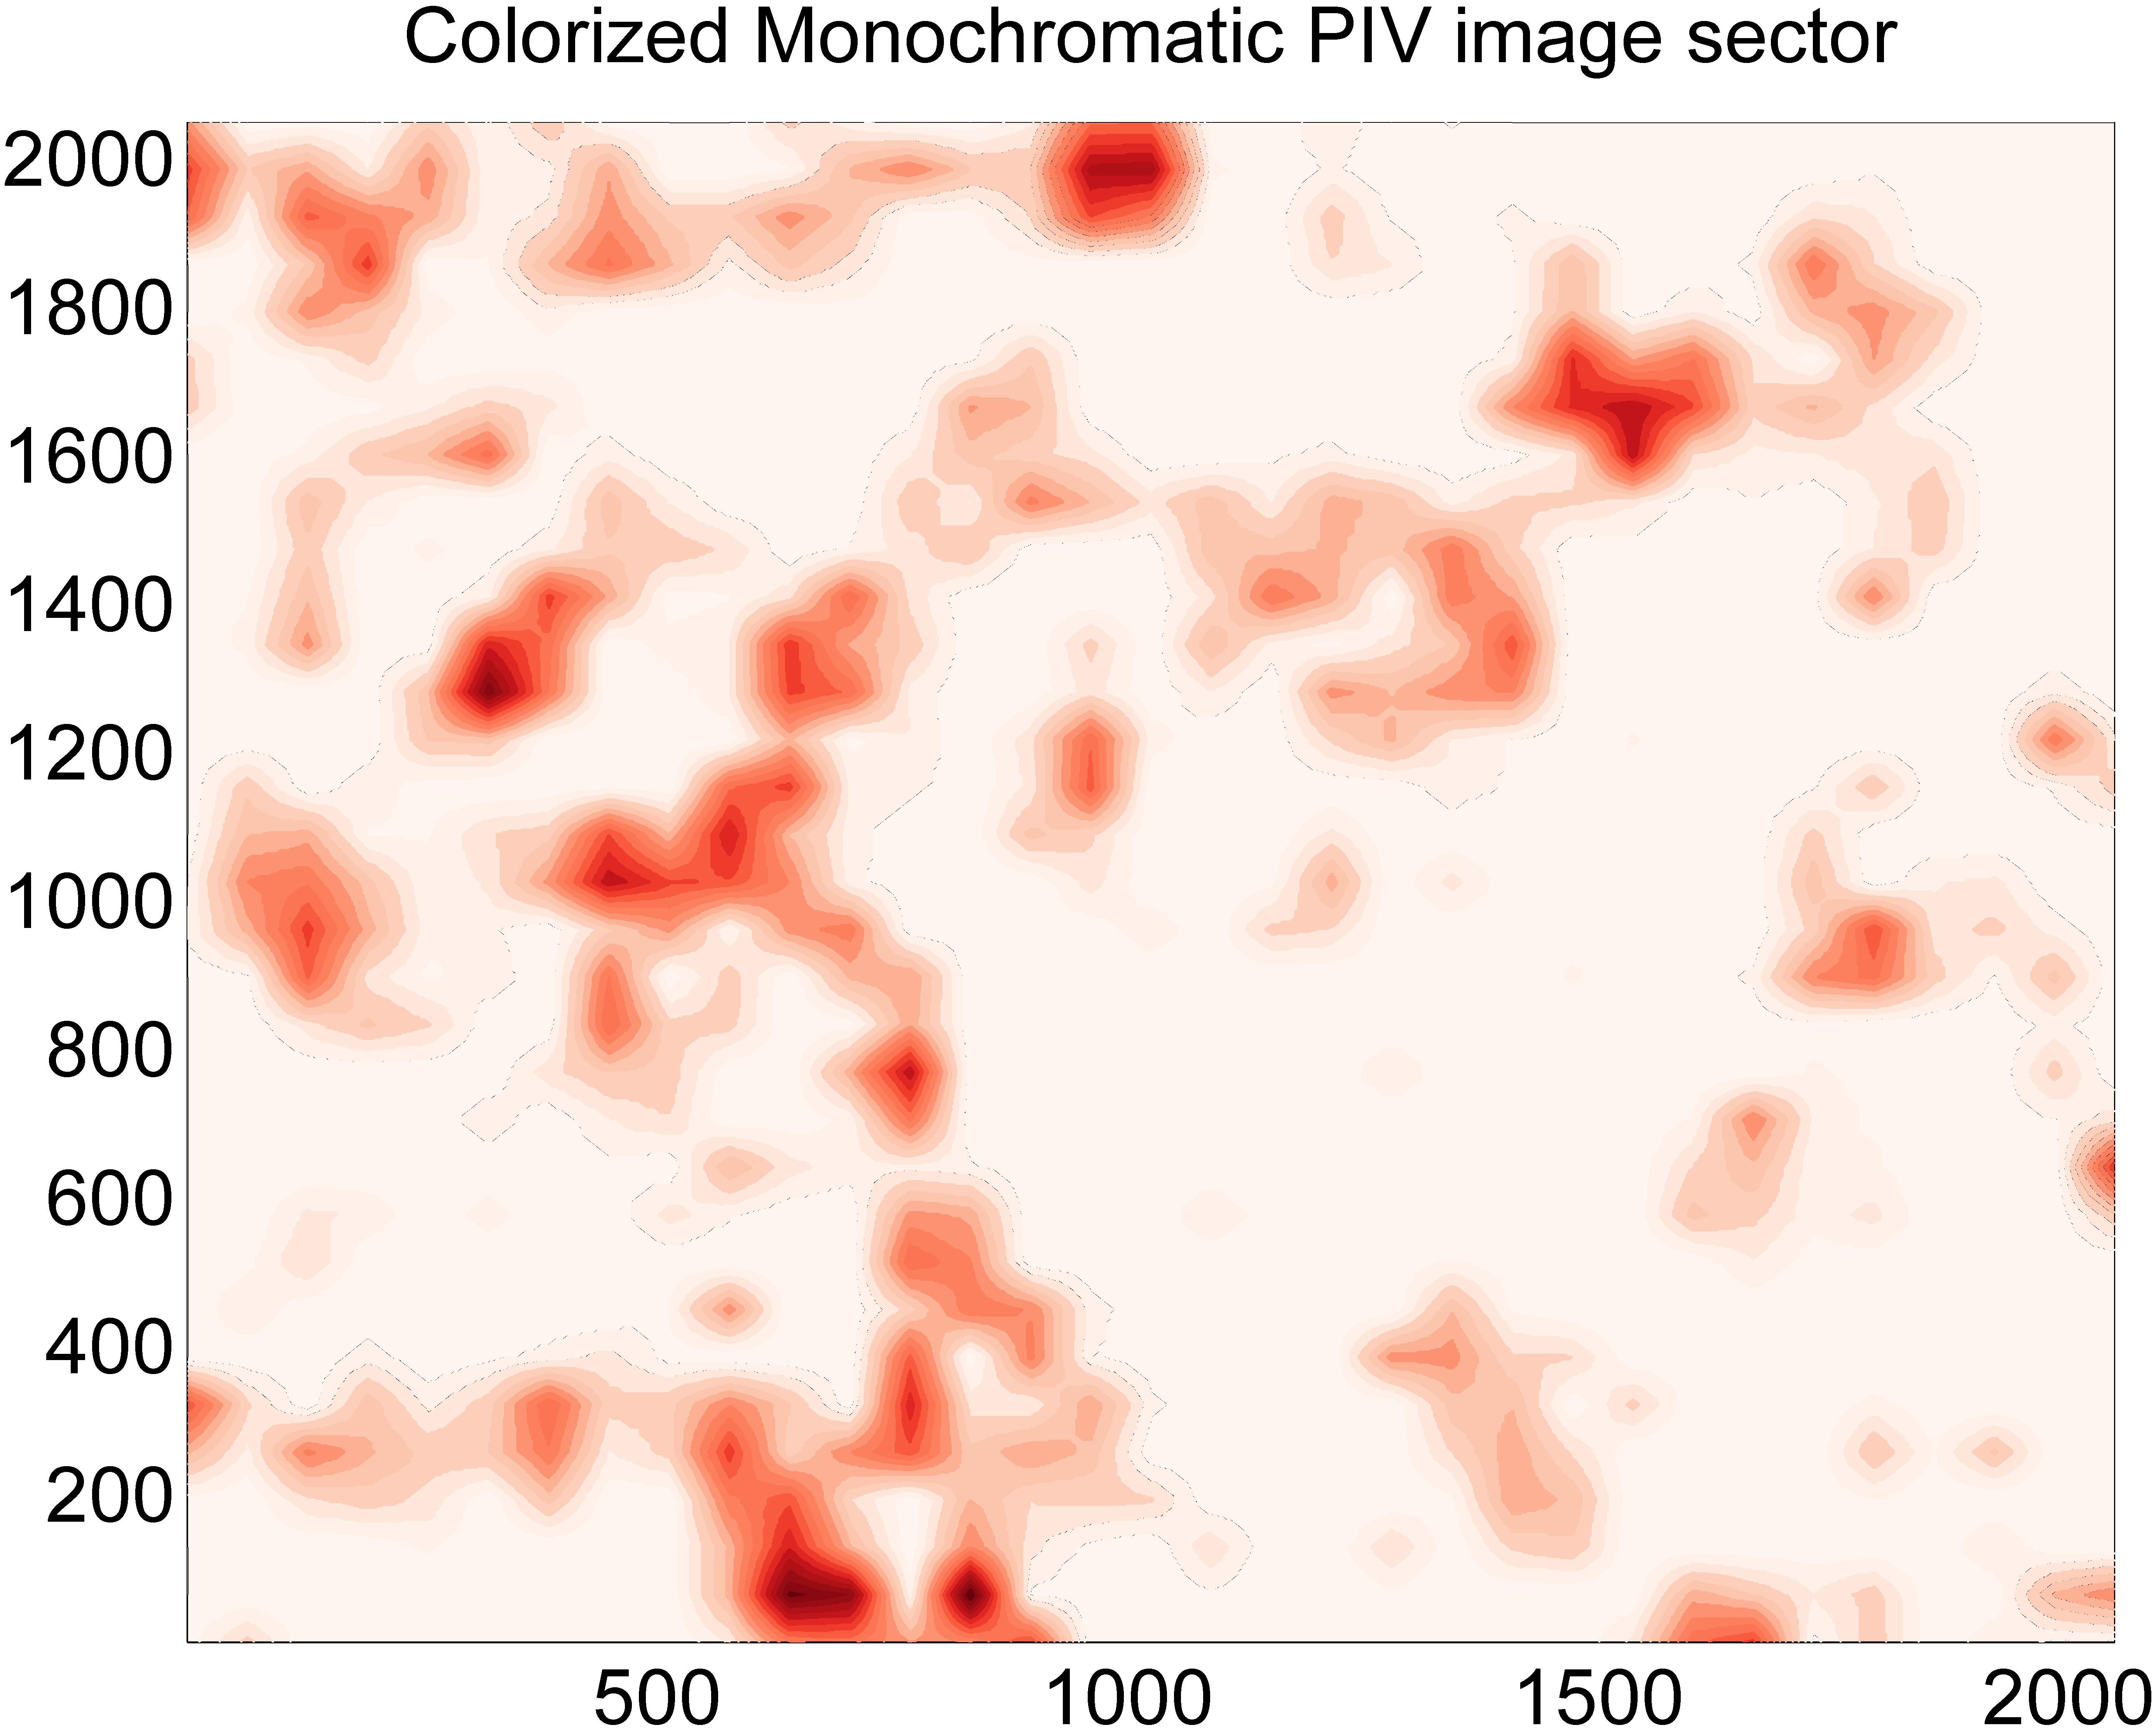
\includegraphics[width=.9\linewidth]{figs/piv_method/pive_figa_order6}
	\end{subfigure} 
	\begin{subfigure}{.49\textwidth}
		\centering
		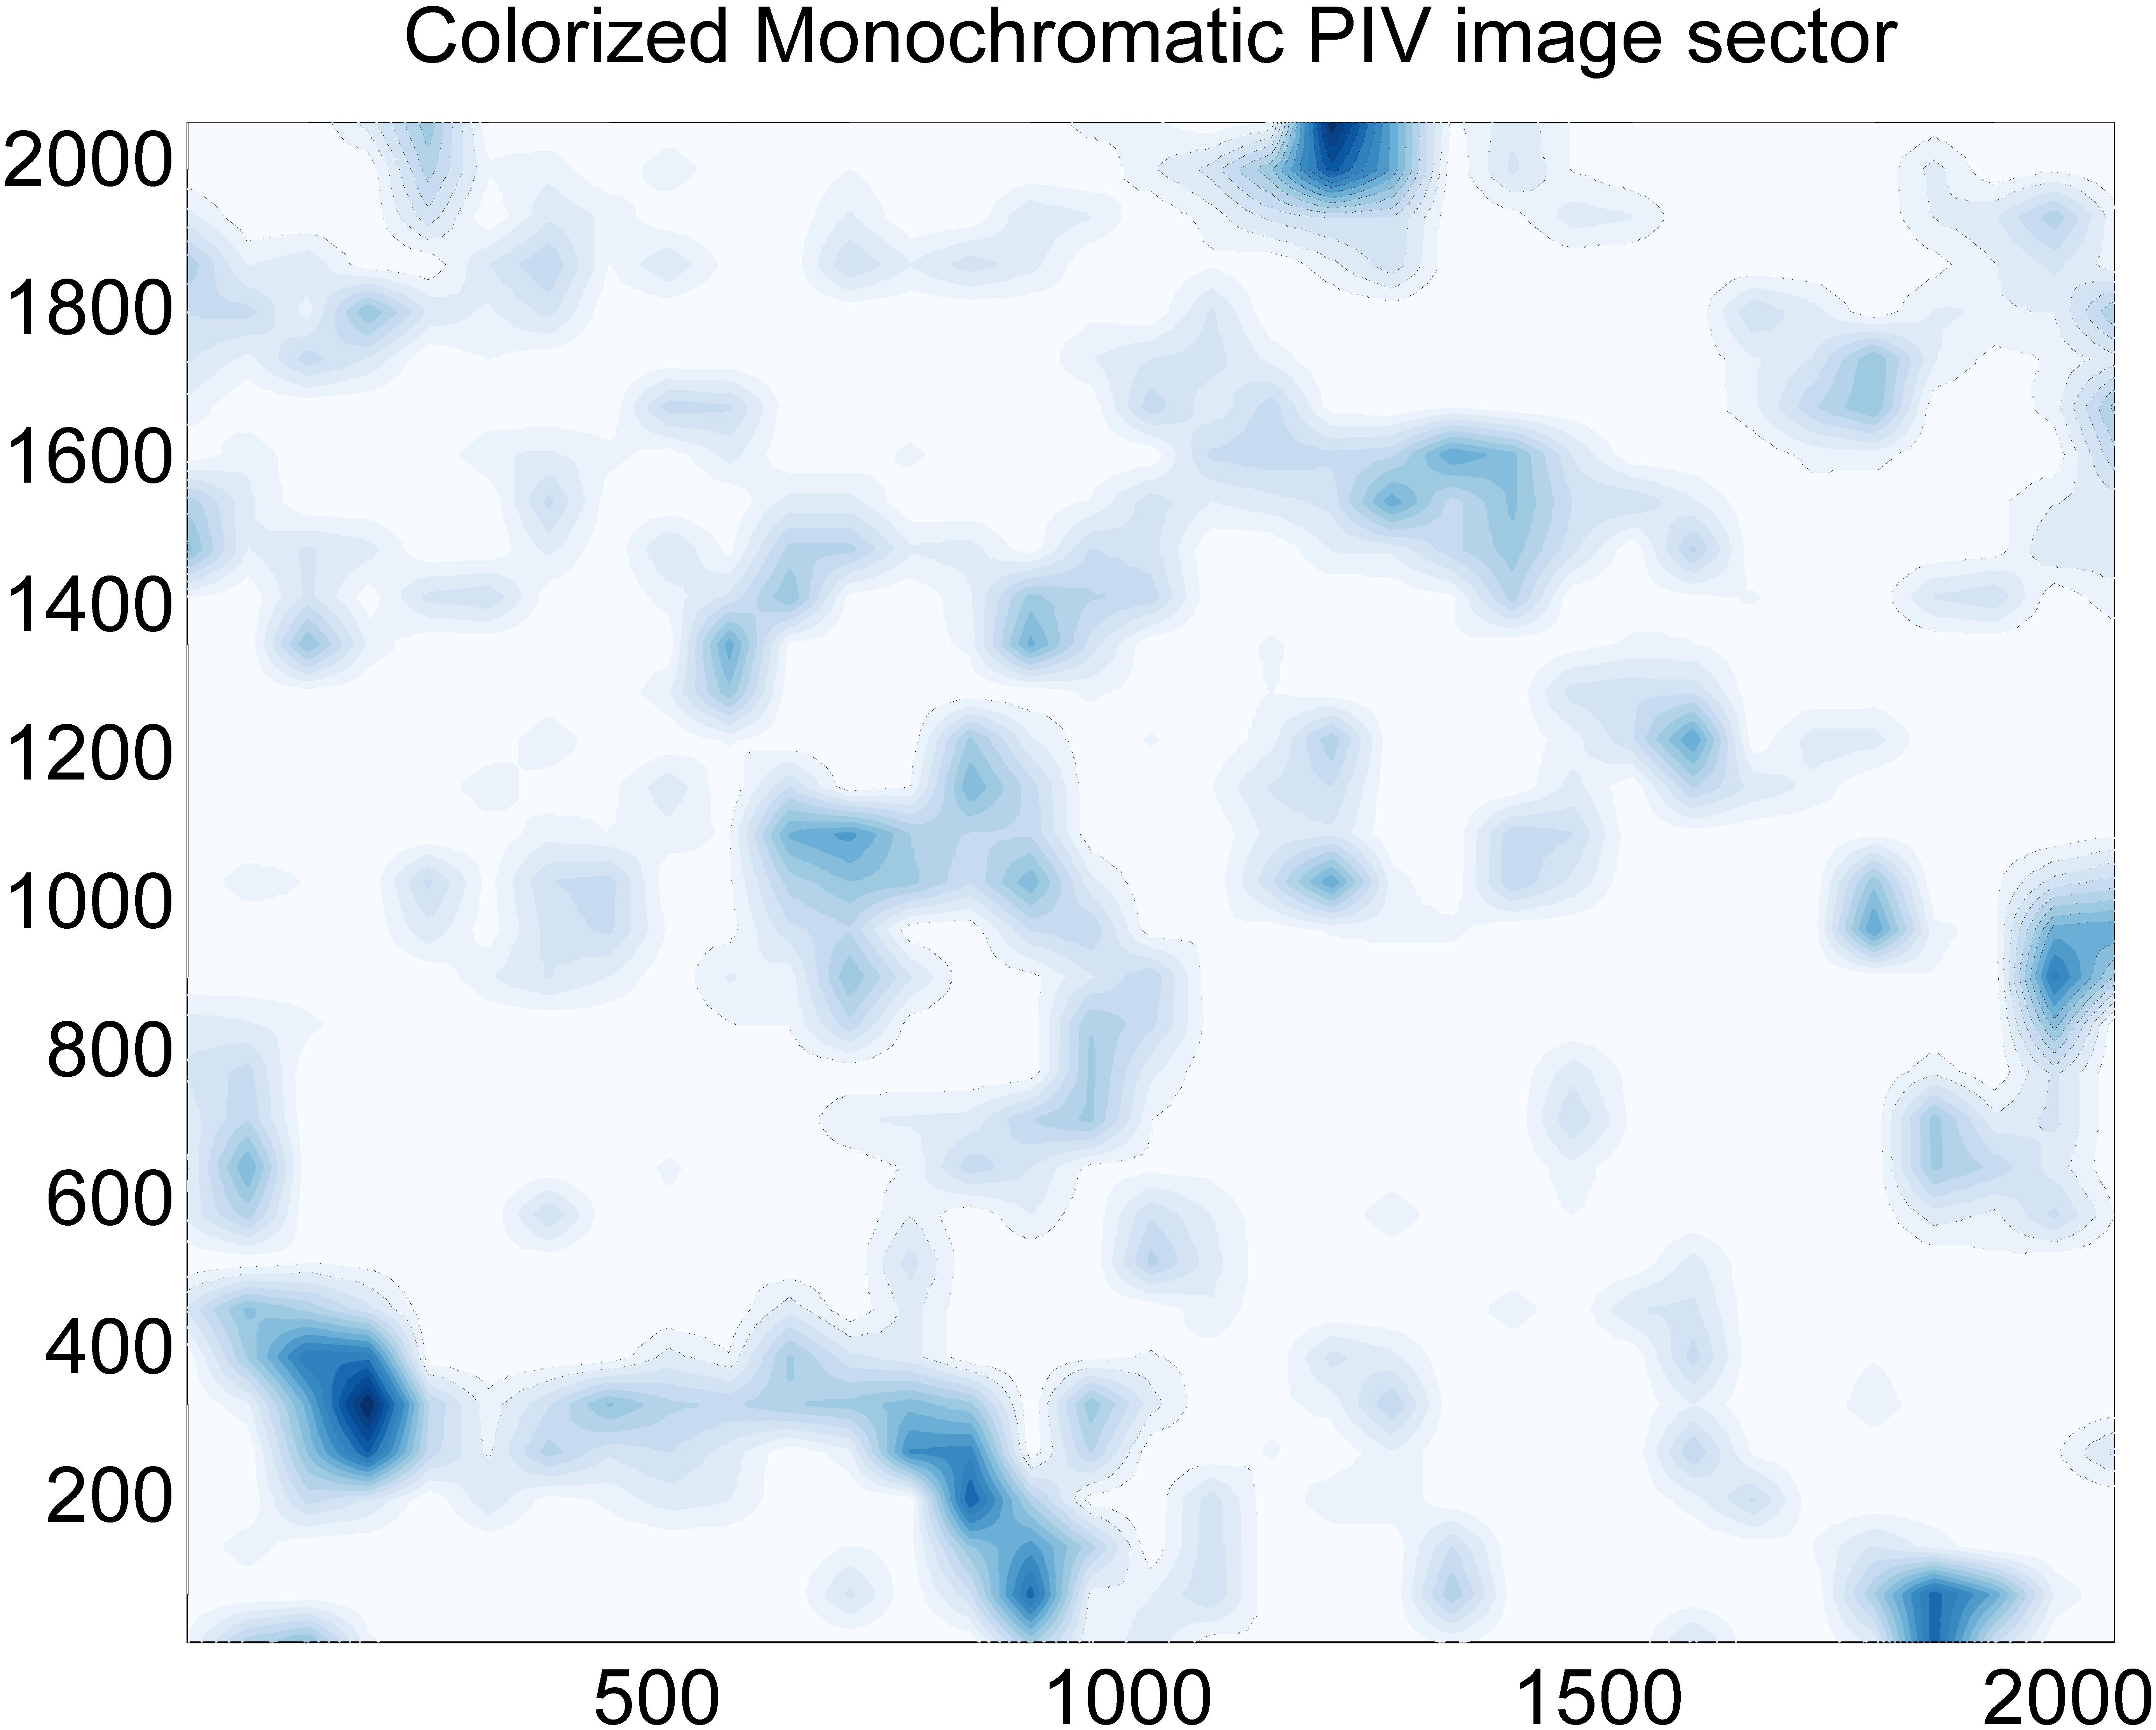
\includegraphics[width=.9\linewidth]{figs/piv_method/pive_figb_order6}
	\end{subfigure}	
	\caption{Colorized 32x32 pixel contour images at $t=0$ (left), and $t=dt$ 
		(right), 6th order up sampling.}
	\label{fig:piv_sector_6up}
\end{figure}


\begin{figure}[H]
	\begin{subfigure}{.49\textwidth}
		\centering
		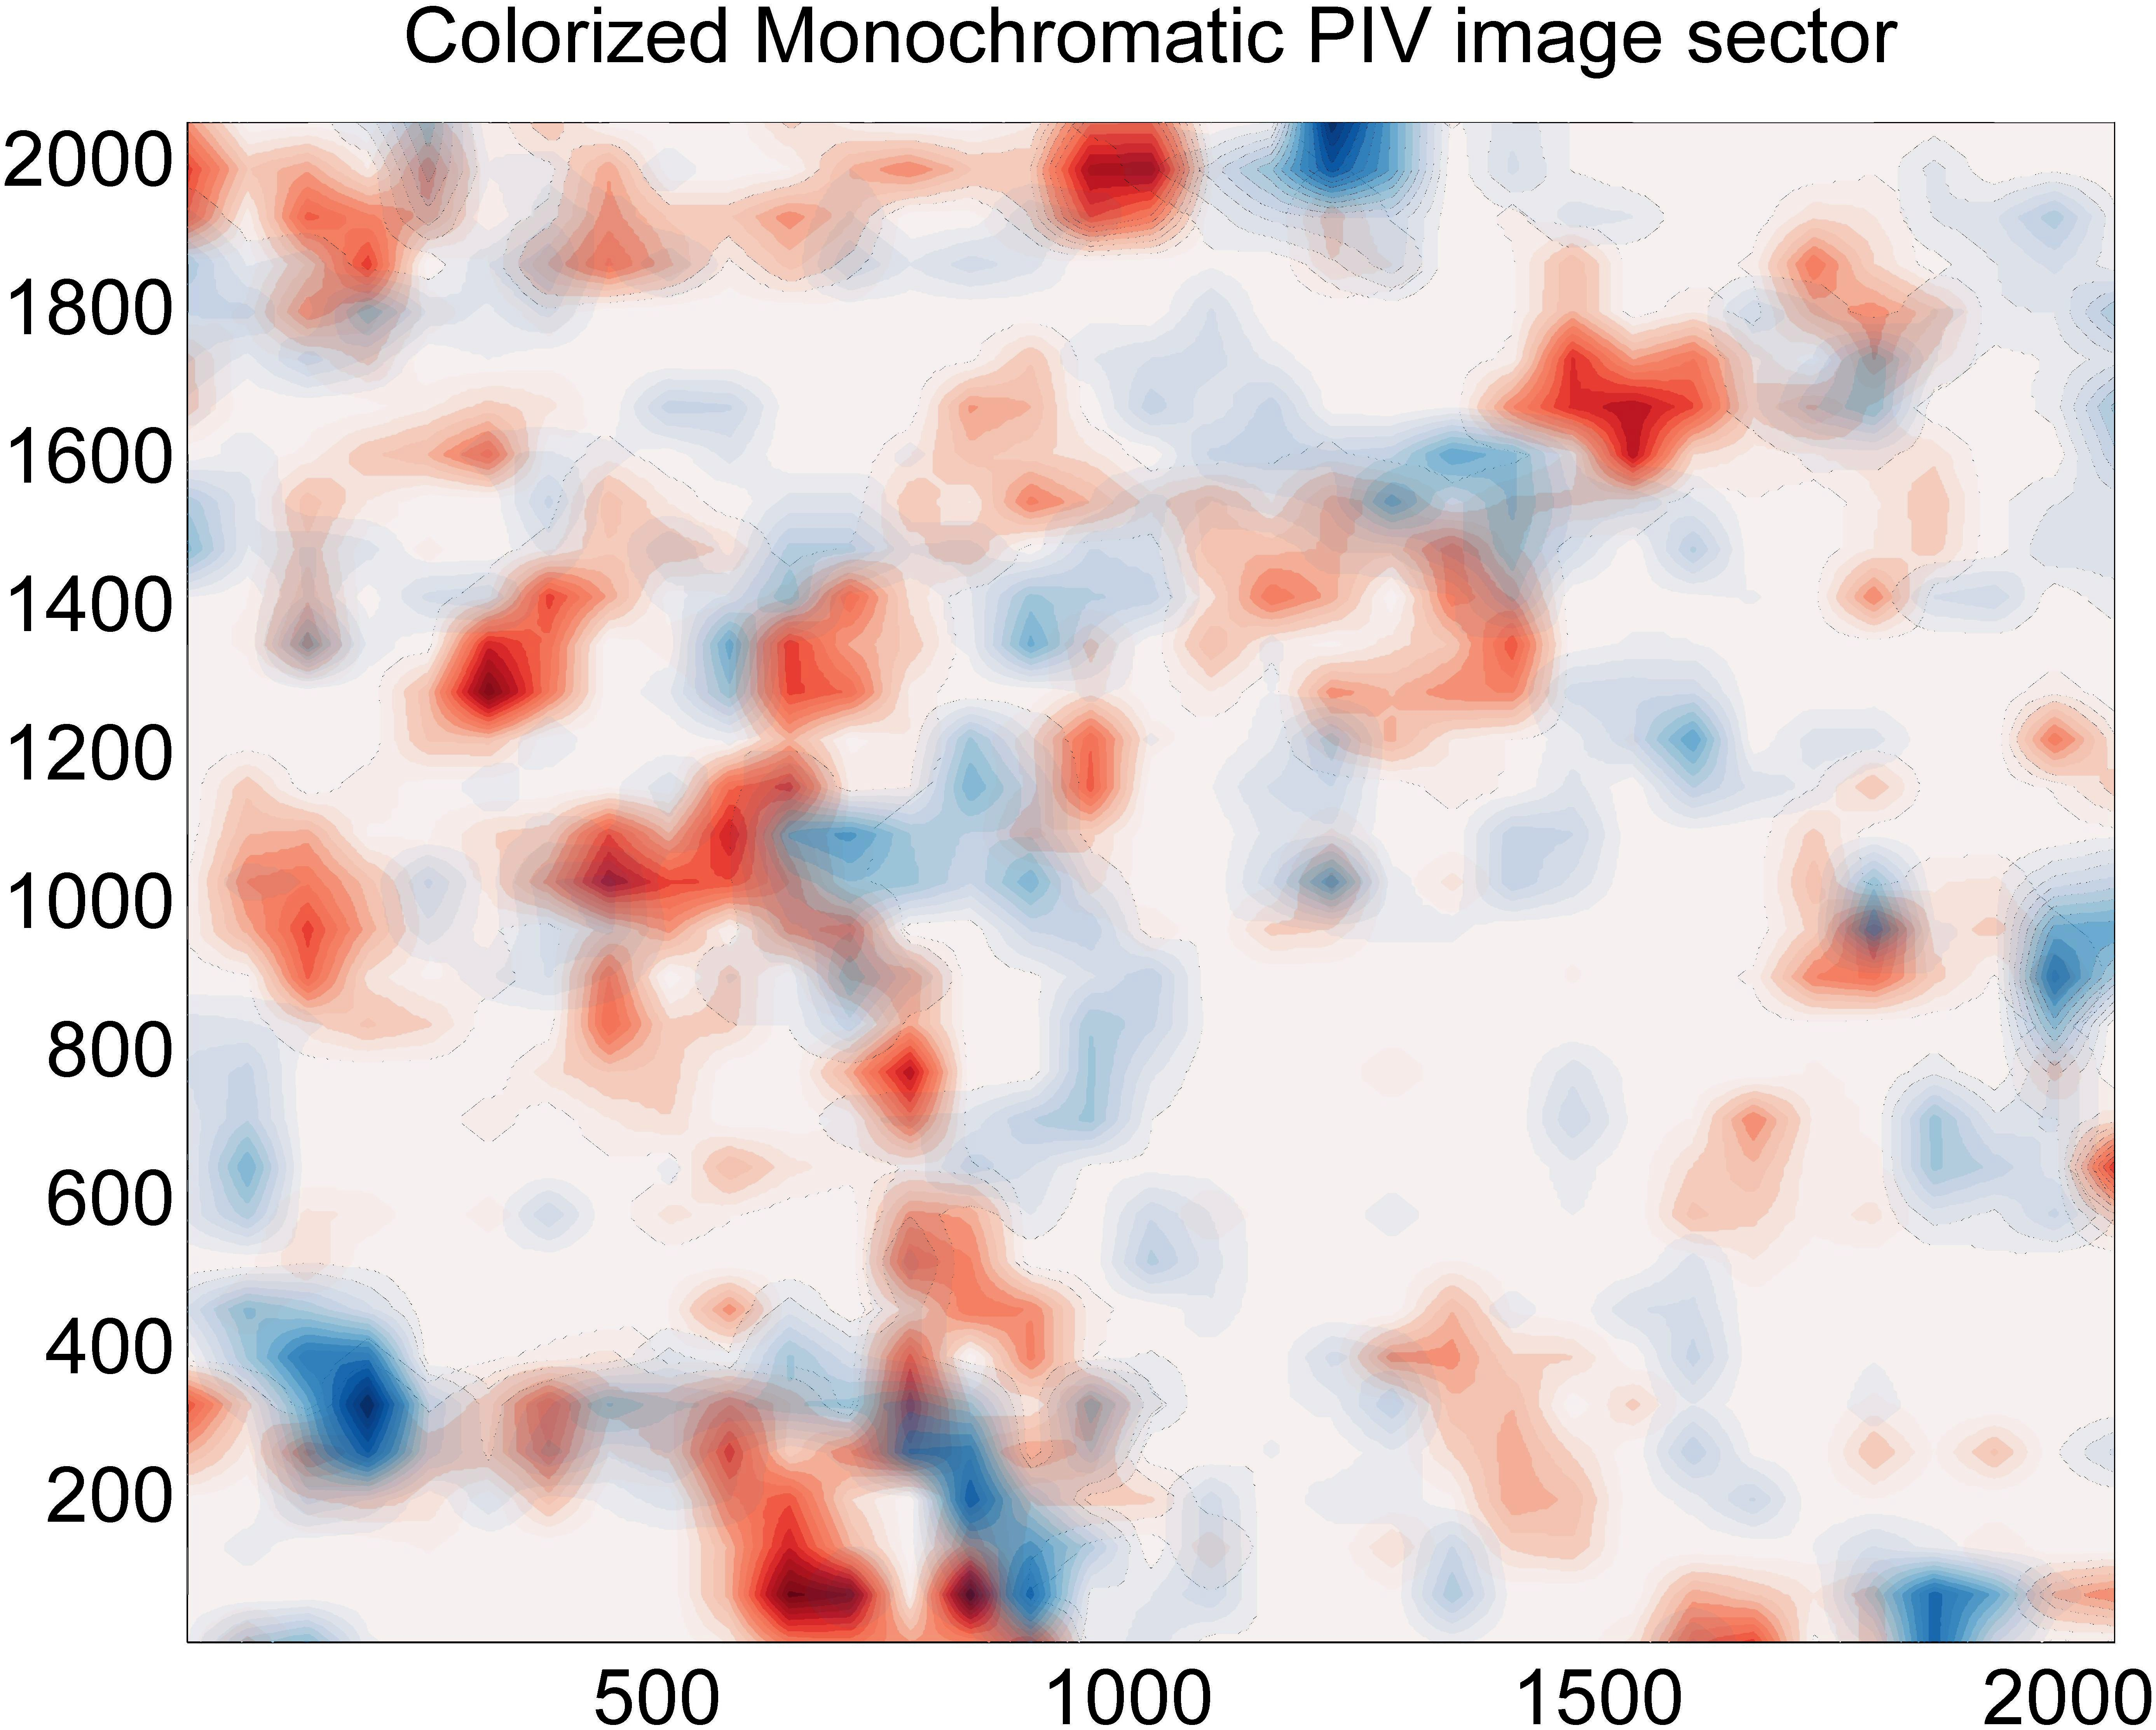
\includegraphics[width=.9\linewidth]{figs/piv_method/pive-fig_order6}
	\end{subfigure} 
	\begin{subfigure}{.49\textwidth}
		\centering
		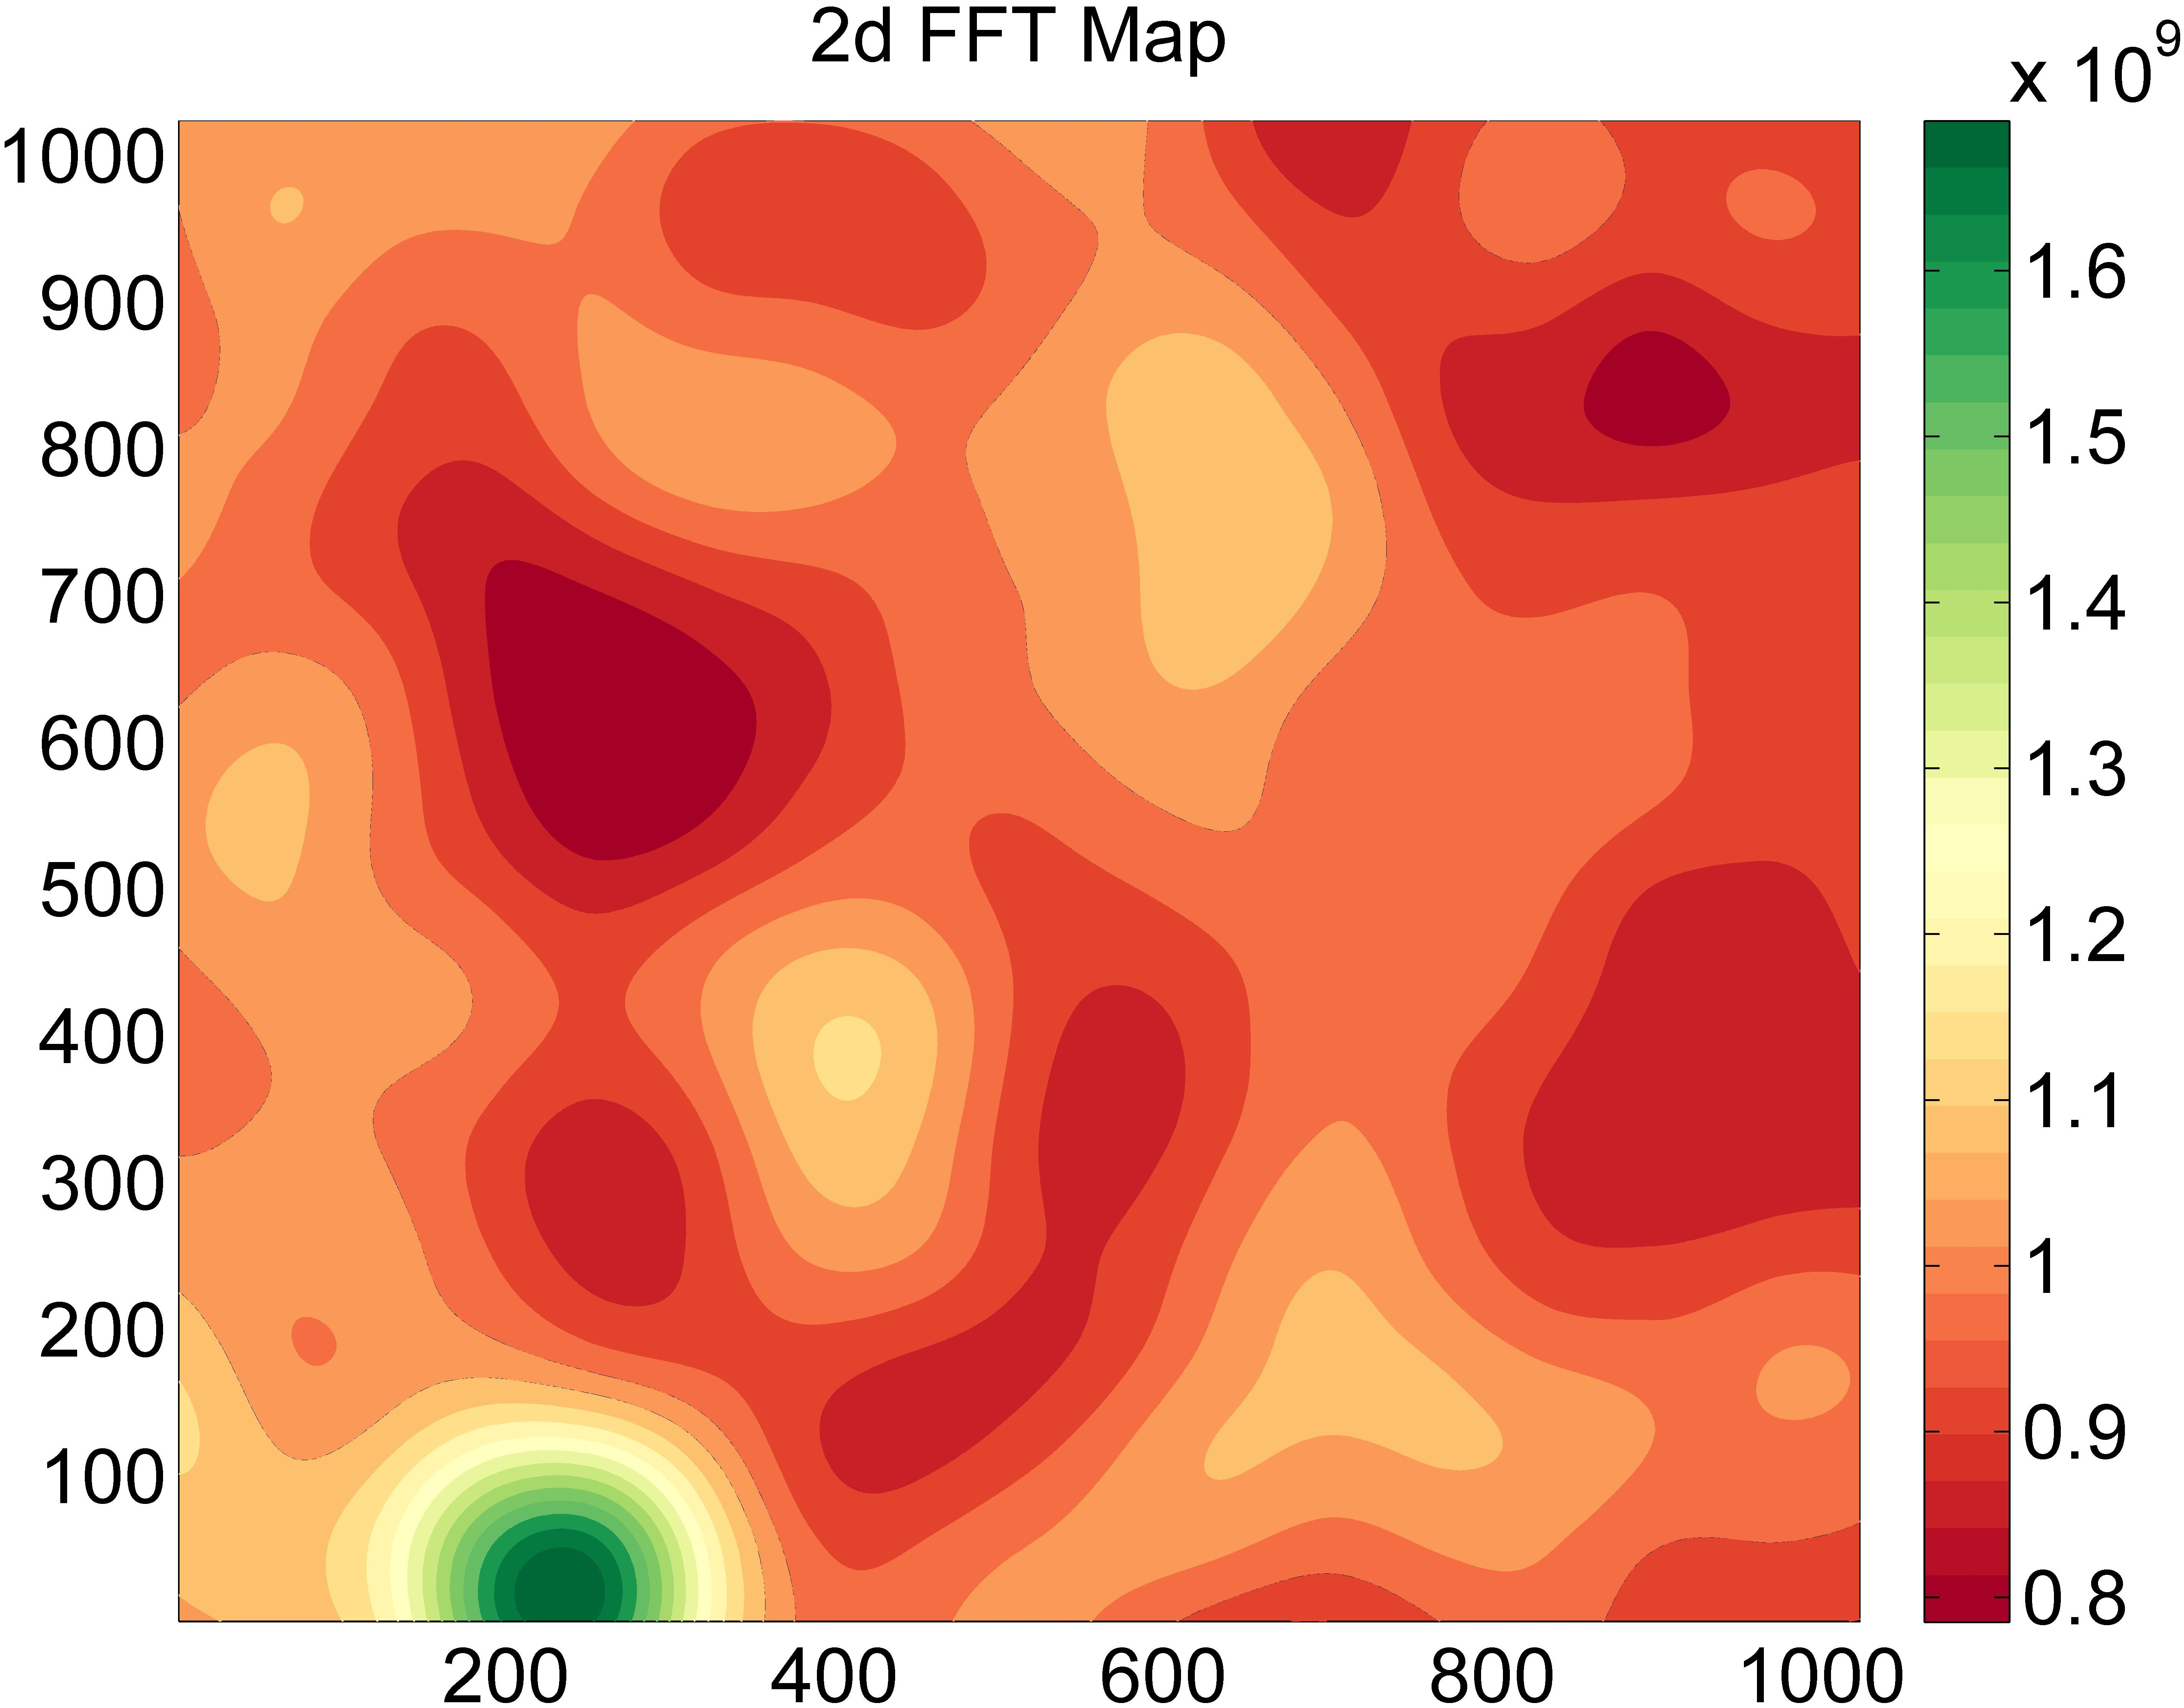
\includegraphics[width=.9\linewidth]{figs/piv_method/pive_fft_order6}
	\end{subfigure}	
	\caption{Overlaid sector snapshots (left) and corresponding correlation 
		map (right), 6th order up sampling.}
	\label{fig:piv_sector_overlay_fft_6up}
\end{figure}

As the sampling method creates a finer mesh, the sub-pixel resolution 
increases. Table \ref{table:piv_upsampling_displacement} shows how the 
displacement error may vary with sampling order.

\begin{table}[H]
\begin{center}
\begin{tabular}{|ccc|}
	\hline
	Order & $x_{disp}$ & $y_{disp}$\\
	\hline
	0 & 4 & 0\\
	1 & 3.5 & 0.5\\
	2 & 3.75 & 0.25\\
	3 & 3.625 & 0.25\\
	4 & 3.625 & 0.3125\\
	5 & 3.625 & 0.3125\\
	6 & 3.6406 & 0.2969\\
	7 & 3.6406 & 0.2969\\
	\hline
\end{tabular}
\caption{Pixel displacements by up sampling order.}
\label{table:piv_upsampling_displacement}
\end{center}
\end{table}


While the above analysis demonstrates the mathematical motivation behind up 
sampling images before performing a Fourier transform for measuring particle 
displacement, it does not adequately describe the total uncertainty in 
measurements made with particle image velocimetry. The uncertainty associated 
with measurements made with PIV are dependent upon the geometry of the specific 
optical setup used to take the data.

In stereo PIV, Equations \ref{eq:piv_to_real1} to \ref{eq:piv_to_real4} the 
derivative terms which relate displacements in the image plane to displacements 
in the real plane are not constant throughout the entire interrogation plane, 
but are functions of the pixels position. These functions can be determined by 
measurement of a calibration target, which has a pattern of dots of known 
position \cite{fouras2007}. The known position of these calibration points can 
be used to compute the nine coefficients for four functions of the form in 
Equation \ref{eq:calibration_equation}. There exists a separate set of nine 
coefficients for the left and right camera, in the $X$ and $Y$ directions.

\begin{equation}
	\begin{multlined}
	X_{mm} =  [A + B(X_{px}) + C(Y_{px}) + D(Z_{mm}) + E(X_{px}^2) + \\
	F(Y_{px}^2) + G(X_{px}Z_{mm}) + H(Y_{px}Z_{mm}) + J(X_{px}Y_{px})]
	\end{multlined}
	\label{eq:calibration_equation}
\end{equation}
\newline
\noindent
where $X_{mm}$ is the position in $mm$, $[A, B, C, D, E, F, G, H, J]$ 
represents the entire set of nine coefficients, $X_{px} and Y_{px}$ are the 
pixel positions in the $X$ and $Y$ directions of the camera plane 
respectively. And $Z_{mm}$ is the actual position in the $Z$ direction. The 
$Z_{mm}$ position of all particles is assumed to be zero in the first image, 
and is determined relative to its starting position by root mean squared of 
the solutions to Equations \ref{eq:piv_to_real1} to \ref{eq:piv_to_real4}.
For simple optical setups, this approach also accounts for distortion due to 
variations in magnification \cite{soloff1997, willert1997}.

\subsection{Uncertainty in PIV}

Understanding the uncertainty in a PIV measurement can be accomplished with 
analysis of the PIV optical geometry \cite{lawson1997b}. Alternatively, Monte 
Carlo techniques for evaluating PIV uncertainty can be used by creating 
artificial image pairs with simulated particle displacements and passing them 
through the PIV processing chain. In PIV, each camera will have a set of 
equations which allow pixel coordinates to be mapped to coordinates of the 
interrogation plane. Particles are simulated with random coordinates within the 
views of both cameras in the interrogation plane, then mapped onto the 
coordinate system of both cameras. The intensity of each pixel can be 
determined by summing the intensity function of every randomly generated 
particle as in \cite{adeyinka2005,fouras2007}.





